\chapter{Quantum Computation Basics}
\label{ch:lec01}

\begin{objectives}
\begin{itemize}[leftmargin=1.4em,nosep]
  \item State the postulates of quantum mechanics in the language of qubits and registers.
  \item Manipulate multi-qubit states via tensor products and Dirac notation.
  \item Read and build simple quantum circuits from a universal gate set.
  \item Build a reversible binary adder from CNOT and Toffoli gates.
  \item Prepare states by gate synthesis and describe projective and generalized (POVM) measurements.
  \item Trace the quantum teleportation and superdense-coding protocols amplitude by amplitude.
  \item Explain measurement, the no-cloning theorem, no-signaling, and density operators.
  \item Quantify nonlocality through the CHSH inequality and its quantum value $2\sqrt2$.
  \item Define the basic complexity measures for quantum algorithms.
\end{itemize}
\end{objectives}

\coverage{\S1.1, \S1.2 (excluding \S1.2.4), \S1.3, \S1.4, \S1.5.1, and \S1.6. Not
covered this term: \S1.2.4 (nonlocality and the CHSH inequality), \S1.5.2 (superdense
coding), \S1.7 (density operators and mixed states), and \S1.8 (complexity of quantum
algorithms).}

This lecture develops the mathematical stage on which all of quantum computing
takes place. The single postulate we need is deceptively simple: \emph{the state
of a quantum system is a unit vector in a complex inner-product space.} From this
one idea we recover Dirac's bra--ket notation, the geometry of overlaps and
orthogonality, the description of a single qubit and the Bloch sphere, and---via
the tensor product---the exponentially large state space of many qubits, where
entanglement first appears. We then turn to the operational layer: gates as
unitary operators, the standard single- and multi-qubit gates, quantum circuits,
universal gate sets, and the no-cloning theorem. We close with two ideas that
recur throughout the course: the density-operator formalism, which lets us
describe subsystems and mixtures, and the complexity measures (query complexity,
gate count, circuit depth) by which we judge quantum algorithms. Everything in
later lectures is built on top of this vocabulary.

\section{Qubits, superposition, and measurement}
\label{sec:lec01-1}

We begin with the linear-algebraic setting.

\begin{definition}[Complex inner-product space]\label{def:lec01-inner}
Let $\Hilb$ be a complex vector space. An \emph{inner product} on $\Hilb$ is a map
$\langle\,\cdot\,,\,\cdot\,\rangle:\Hilb\times\Hilb\to\C$ satisfying, for all
$u,v,w\in\Hilb$ and $a,b\in\C$:
\begin{enumerate}[label=(\roman*)]
  \item \emph{Conjugate symmetry:} $\langle u,v\rangle=\overline{\langle v,u\rangle}$.
  \item \emph{Linearity in the second argument:}
        $\langle u,\,a v+b w\rangle=a\langle u,v\rangle+b\langle u,w\rangle$.
        (Combined with (i), this makes the inner product \emph{conjugate-linear}
        in the first argument.)
  \item \emph{Positive-definiteness:} $\langle u,u\rangle\ge 0$, with equality
        if and only if $u=0$.
\end{enumerate}
\end{definition}

We adopt the physicists' convention that the inner product is linear in the
\emph{second} slot and conjugate-linear in the first; this is the convention that
makes Dirac notation come out cleanly. Concretely, on $\C^{N}$ with
$x=(x_0,\dots,x_{N-1})^{T}$ and $y=(y_0,\dots,y_{N-1})^{T}$,
\begin{equation}
  \langle x,y\rangle \;=\; x\dg y \;=\; \sum_{i=0}^{N-1}\overline{x_i}\,y_i .
\end{equation}

\begin{definition}[Norm and unit vector]\label{def:lec01-norm}
The \emph{norm} induced by the inner product is $\norm{u}=\sqrt{\langle u,u\rangle}$.
A vector $u$ is a \emph{unit vector} (or \emph{normalized}) if $\norm{u}=1$. Two
vectors $u,v$ are \emph{orthogonal} if $\langle u,v\rangle=0$.
\end{definition}

\begin{definition}[Finite-dimensional Hilbert space]\label{def:lec01-hilbert}
A \emph{finite-dimensional Hilbert space} is a finite-dimensional complex
inner-product space $\Hilb$ (in finite dimension completeness is automatic, so no
further condition is needed). If $\dim\Hilb=N$, then choosing an orthonormal basis
gives an isomorphism $\Hilb\cong\C^{N}$ that preserves the inner product. For a
system of $n$ qubits we will find $N=2^{n}$.
\end{definition}

The state-space postulate can now be stated precisely.

\begin{remark}[State-space postulate]
The state of an isolated quantum system is described by a \emph{unit} vector in a
Hilbert space $\Hilb$. The space is closed under linear combination: if
$u,v\in\Hilb$ and $a,b\in\C$, then $a u+b v\in\Hilb$. This closure is the
\emph{superposition principle}---any linear combination of legal states is again a
legal (unnormalized) state.
\end{remark}

\subsection{The inner product controls all geometry}

\begin{proposition}[Elementary consequences of the axioms]\label{prop:lec01-elem}
For all $u,v\in\Hilb$ and $a\in\C$:
\begin{enumerate}[label=(\alph*)]
  \item $\langle u,0\rangle=\langle 0,u\rangle=0$;
  \item $\norm{a u}=\abs{a}\,\norm{u}$;
  \item \emph{(Pythagoras)} if $\langle u,v\rangle=0$ then
        $\norm{u+v}^{2}=\norm{u}^{2}+\norm{v}^{2}$.
\end{enumerate}
\end{proposition}

\begin{proof}
(a) By linearity in the second argument, $\langle u,0\rangle=\langle u,0\cdot 0\rangle=0\,\langle u,0\rangle=0$;
the other equality follows from conjugate symmetry.
(b) $\norm{a u}^{2}=\langle a u,a u\rangle=\overline{a}\,a\,\langle u,u\rangle=\abs{a}^{2}\norm{u}^{2}$,
and take square roots.
(c) Expand $\norm{u+v}^{2}=\langle u+v,u+v\rangle=\norm{u}^{2}+\langle u,v\rangle+\langle v,u\rangle+\norm{v}^{2}$;
the two cross terms vanish because $\langle u,v\rangle=0$ forces
$\langle v,u\rangle=\overline{\langle u,v\rangle}=0$.
\end{proof}

The single most useful inequality in the whole subject is the following.

\begin{theorem}[Cauchy--Schwarz inequality]\label{thm:lec01-cs}
For all $u,v\in\Hilb$,
\begin{equation}
  \abs{\langle u,v\rangle}\;\le\;\norm{u}\,\norm{v},
\end{equation}
with equality if and only if $u$ and $v$ are linearly dependent.
\end{theorem}

\begin{proof}
If $v=0$ both sides are $0$ and $u,v$ are trivially dependent, so assume $v\neq0$.
For any $\lambda\in\C$, positive-definiteness gives
\[
  0\;\le\;\norm{u-\lambda v}^{2}
   \;=\;\norm{u}^{2}-\overline{\lambda}\langle v,u\rangle-\lambda\langle u,v\rangle+\abs{\lambda}^{2}\norm{v}^{2}.
\]
Choose $\lambda=\dfrac{\langle v,u\rangle}{\norm{v}^{2}}$ (the value that minimizes the
right-hand side). Then $\lambda\langle u,v\rangle=\dfrac{\langle v,u\rangle\langle u,v\rangle}{\norm{v}^{2}}=\dfrac{\abs{\langle u,v\rangle}^{2}}{\norm{v}^{2}}$, and likewise $\overline{\lambda}\langle v,u\rangle=\dfrac{\abs{\langle u,v\rangle}^{2}}{\norm{v}^{2}}$, so
\[
  0\;\le\;\norm{u}^{2}-\frac{\abs{\langle u,v\rangle}^{2}}{\norm{v}^{2}}.
\]
Rearranging yields $\abs{\langle u,v\rangle}^{2}\le\norm{u}^{2}\norm{v}^{2}$, i.e.
the claim. Equality holds iff $\norm{u-\lambda v}=0$, i.e. $u=\lambda v$, which is
exactly linear dependence.
\end{proof}

\begin{corollary}[Triangle inequality]\label{cor:lec01-tri}
$\norm{u+v}\le\norm{u}+\norm{v}$ for all $u,v\in\Hilb$.
\end{corollary}

\begin{proof}
$\norm{u+v}^{2}=\norm{u}^{2}+2\,\mathrm{Re}\,\langle u,v\rangle+\norm{v}^{2}
 \le \norm{u}^{2}+2\abs{\langle u,v\rangle}+\norm{v}^{2}
 \le \norm{u}^{2}+2\norm{u}\norm{v}+\norm{v}^{2}=(\norm{u}+\norm{v})^{2}$,
using $\mathrm{Re}\,z\le\abs{z}$ and \cref{thm:lec01-cs}. Take square roots.
\end{proof}

For unit vectors the Cauchy--Schwarz inequality reads $\abs{\langle u,v\rangle}\le1$,
so we may write
\begin{equation}\label{eq:lec01-geomdecomp}
  \langle u,v\rangle \;=\; \underbrace{\norm{u}\,\norm{v}}_{\text{length}}\;
  \underbrace{\cos\theta}_{\text{alignment}}\;\underbrace{\ee^{\ii\varphi}}_{\text{relative phase}},
  \qquad \cos\theta=\frac{\abs{\langle u,v\rangle}}{\norm{u}\,\norm{v}}\in[0,1].
\end{equation}
The modulus measures how much the two directions coincide ($\cos\theta=1$ means
parallel, $\cos\theta=0$ means orthogonal), while the argument $\varphi$ is a
\emph{relative phase} with no analogue for real vectors. Orthogonality,
$\langle u,v\rangle=0$, is exactly the statement that the two states are perfectly
distinguishable.

\subsection{Dirac notation}

\begin{definition}[Ket and bra]\label{def:lec01-braket}
A vector of $\Hilb$ is written as a \emph{ket} $\ket{x}$. To each ket there
corresponds a \emph{bra} $\bra{x}$, the element of the dual space $\Hilb^{*}$
acting by $\bra{x}:\ket{y}\mapsto\langle x,y\rangle$. In coordinates, if $\ket{x}$
is the column vector with entries $x_i$, then $\bra{x}$ is the row vector
$x\dg=(\overline{x_0},\dots,\overline{x_{N-1}})$, the conjugate transpose.
\end{definition}

\begin{definition}[Inner and outer products]\label{def:lec01-inout}
The \emph{inner product} of $\ket{x}$ and $\ket{y}$ is the scalar
$\braket{x|y}=\langle x,y\rangle\in\C$. The \emph{outer product} $\ket{x}\!\bra{y}$
is the linear operator acting as
\[
  \bigl(\ket{x}\!\bra{y}\bigr)\ket{z}=\ket{x}\,\braket{y|z}=\braket{y|z}\,\ket{x}.
\]
In coordinates it is the matrix with entries $\bigl(\ket{x}\!\bra{y}\bigr)_{ij}=x_i\,\overline{y_j}$.
\end{definition}

Fix an orthonormal basis $\{\ket{i}\}_{i=0}^{N-1}$, meaning $\braket{i|j}=\delta_{ij}$.
Any ket expands as $\ket{x}=\sum_i x_i\ket{i}$, and applying $\bra{j}$ picks out a
single coefficient:
\begin{equation}\label{eq:lec01-coeff}
  \braket{j|x}=\sum_i x_i\braket{j|i}=\sum_i x_i\,\delta_{ji}=x_j .
\end{equation}
So the $j$-th amplitude is literally the overlap $\braket{j|x}$.

\begin{theorem}[Completeness / resolution of the identity]\label{thm:lec01-completeness}
If $\{\ket{i}\}_{i=0}^{N-1}$ is an orthonormal basis of $\Hilb$, then
\begin{equation}
  \sum_{i=0}^{N-1}\proj{i}\;=\;\id .
\end{equation}
Consequently every operator $A$ satisfies $A=\sum_{i,j}A_{ij}\,\ket{i}\!\bra{j}$ with
$A_{ij}=\braket{i|A|j}$.
\end{theorem}

\begin{proof}
Let $P=\sum_i\proj{i}$. For an arbitrary $\ket{x}=\sum_j x_j\ket{j}$,
\[
  P\ket{x}=\sum_i\ket{i}\braket{i|x}=\sum_i x_i\ket{i}=\ket{x},
\]
using \eqref{eq:lec01-coeff}. Since $P\ket{x}=\ket{x}$ for every $\ket{x}$, we have
$P=\id$. For the second statement, insert the identity on both sides of $A$:
$A=\id\,A\,\id=\sum_{i,j}\ket{i}\braket{i|A|j}\bra{j}=\sum_{i,j}A_{ij}\,\ket{i}\!\bra{j}$.
\end{proof}

\begin{remark}[Projectors]
For a unit vector $\ket{u}$ the operator $P_u=\proj{u}$ is the orthogonal
\emph{projector} onto the line spanned by $\ket{u}$: it is Hermitian
($P_u\dg=P_u$) and idempotent, since $P_u^{2}=\ket{u}\braket{u|u}\bra{u}=\proj{u}=P_u$
because $\braket{u|u}=1$. The completeness relation of
\cref{thm:lec01-completeness} decomposes $\id$ into a sum of orthogonal rank-one
projectors, one per basis vector.
\end{remark}

\subsection{The single qubit}

\begin{definition}[Qubit and computational basis]\label{def:lec01-qubit}
A \emph{qubit} is a quantum system whose state space is $\Hilb=\C^{2}$. The
distinguished orthonormal basis
\[
  \ket{0}=\begin{pmatrix}1\\0\end{pmatrix},\qquad
  \ket{1}=\begin{pmatrix}0\\1\end{pmatrix}
\]
is called the \emph{computational basis}. A general pure state is
\begin{equation}\label{eq:lec01-qubit}
  \ket{\psi}=a\ket{0}+b\ket{1},\qquad a,b\in\C,\qquad \abs{a}^{2}+\abs{b}^{2}=1 .
\end{equation}
The coefficients $a,b$ are called \emph{amplitudes}; $\abs{a}^{2}$ and $\abs{b}^{2}$
are the probabilities of obtaining $0$ or $1$ in a computational-basis measurement.
\end{definition}

The recipe just stated---outcome $i$ occurs with probability $\abs{\braket{i|\psi}}^{2}$,
and the post-measurement state collapses to $\ket{i}$---is the \emph{Born rule},
the measurement postulate of quantum mechanics. More generally, a projective
measurement with orthogonal projectors $\{P_m\}$, $\sum_m P_m=\id$, returns outcome
$m$ with probability $p_m=\bra{\psi}P_m\ket{\psi}$ and leaves the state
$P_m\ket{\psi}/\sqrt{p_m}$; the probabilities sum to one by completeness.

\begin{remark}[Global phase is unobservable]\label{rem:lec01-global}
Measurement probabilities depend on the amplitudes only through moduli of the form
$\abs{\braket{i|\psi}}^{2}$. Replacing $\ket{\psi}$ by $\ee^{\ii\gamma}\ket{\psi}$ for a
real \emph{global phase} $\gamma$ leaves every such probability unchanged, and more
generally leaves $\braket{\phi|A|\psi}$-type quantities invariant when the same
phase appears on both sides. Hence $\ee^{\ii\gamma}\ket{\psi}$ and $\ket{\psi}$ describe
the same physical state: genuine states are points of the \emph{projective space}
$\Prob(\Hilb)$, i.e. rays rather than vectors. \emph{Relative} phases between the
terms of a superposition, by contrast, are physical and drive interference.
\end{remark}

\begin{proposition}[Bloch parametrization]\label{prop:lec01-bloch}
Every single-qubit pure state can be written, up to an unobservable global phase, as
\begin{equation}\label{eq:lec01-blochform}
  \ket{\psi}=\cos\tfrac{\theta}{2}\,\ket{0}+\ee^{\ii\varphi}\sin\tfrac{\theta}{2}\,\ket{1},
  \qquad \theta\in[0,\pi],\quad \varphi\in[0,2\pi).
\end{equation}
The pair $(\theta,\varphi)$ is the pair of spherical angles of a point on the unit
sphere $S^{2}\subset\R^{3}$, the \emph{Bloch sphere}.
\end{proposition}

\begin{proof}
Start from \eqref{eq:lec01-qubit} with $\abs{a}^{2}+\abs{b}^{2}=1$. Write the
amplitudes in polar form $a=r_a \ee^{\ii\alpha}$ and $b=r_b \ee^{\ii\beta}$ with
$r_a,r_b\ge0$. Since $r_a^{2}+r_b^{2}=1$ we may set $r_a=\cos\tfrac{\theta}{2}$ and
$r_b=\sin\tfrac{\theta}{2}$ for a unique $\theta\in[0,\pi]$ (both cosine and sine of
$\theta/2$ are then nonnegative). Thus
\[
  \ket{\psi}=\ee^{\ii\alpha}\cos\tfrac{\theta}{2}\ket{0}+\ee^{\ii\beta}\sin\tfrac{\theta}{2}\ket{1}
           =\ee^{\ii\alpha}\Bigl(\cos\tfrac{\theta}{2}\ket{0}+\ee^{\ii(\beta-\alpha)}\sin\tfrac{\theta}{2}\ket{1}\Bigr).
\]
The overall factor $\ee^{\ii\alpha}$ is a global phase, which by
\cref{rem:lec01-global} we may discard. Setting $\varphi=\beta-\alpha\ (\mathrm{mod}\ 2\pi)$
gives \eqref{eq:lec01-blochform}. When $\theta\in\{0,\pi\}$ the state is $\ket{0}$
or $\ket{1}$ and $\varphi$ is irrelevant (the poles of the sphere), consistent with
the identification of states with points of $S^{2}$.
\end{proof}

\begin{remark}[Reading the Bloch sphere]
In this picture $\ket{0}$ and $\ket{1}$ sit at the north and south poles
($\theta=0,\pi$), and \emph{orthogonal} qubit states are \emph{antipodal} points,
not perpendicular ones---a state and its orthogonal complement are separated by
angle $\theta=\pi$ on the sphere even though they are separated by $90^{\circ}$ in
$\C^{2}$. The equatorial states $\tfrac{1}{\sqrt2}(\ket{0}+\ee^{\ii\varphi}\ket{1})$
have $\theta=\pi/2$ and differ only in their relative phase $\varphi$.
\end{remark}

\begin{example}[Amplitudes and normalization]\label{ex:lec01-pm}
The state $\ket{+}=\tfrac{1}{\sqrt2}(\ket{0}+\ket{1})$ has
$\abs{a}^{2}=\abs{b}^{2}=\tfrac12$, so a computational-basis measurement yields $0$
or $1$ with equal probability $\tfrac12$; its Bloch angles are $\theta=\pi/2,\varphi=0$.
The state $\ket{-}=\tfrac{1}{\sqrt2}(\ket{0}-\ket{1})$ has the \emph{same} measurement
statistics in the computational basis but differs by the relative phase
$\varphi=\pi$; indeed $\braket{+|-}=\tfrac12(1-1)=0$, so $\ket{+}$ and $\ket{-}$ are
orthogonal and perfectly distinguishable by a suitable measurement.
\end{example}

\section{Multi-qubit systems and tensor products}
\label{sec:lec01-2}

\begin{definition}[Tensor-product state space]\label{def:lec01-tensor}
If systems $A$ and $B$ have state spaces $\Hilb_A$ and $\Hilb_B$, the composite
system has state space the \emph{tensor product} $\Hilb_A\otimes\Hilb_B$. If
$\{\ket{i}_A\}$ and $\{\ket{j}_B\}$ are orthonormal bases, then
$\{\ket{i}_A\otimes\ket{j}_B\}$ is an orthonormal basis of the product, with inner
product
\[
  \bigl(\bra{i}\otimes\bra{j}\bigr)\bigl(\ket{k}\otimes\ket{l}\bigr)
    =\braket{i|k}\,\braket{j|l}.
\]
Hence $\dim(\Hilb_A\otimes\Hilb_B)=(\dim\Hilb_A)(\dim\Hilb_B)$. For $n$ qubits,
\[
  \Hilb=(\C^{2})^{\otimes n}\cong\C^{2^{n}},\qquad \dim\Hilb=2^{n}.
\]
\end{definition}

We abbreviate $\ket{i}\otimes\ket{j}$ as $\ket{i}\ket{j}$ or $\ket{ij}$. The
computational basis of $n$ qubits is $\{\ket{x}:x\in\{0,1\}^{n}\}$, indexed by the
$2^{n}$ bit strings. The exponential growth of the dimension---$50$ qubits already
give a space of dimension $2^{50}>10^{15}$---is one root of quantum computing's
potential power: a classical description of a general state requires exponentially
many amplitudes.

\begin{remark}[The $\ket{k}$ notation for computational-basis states]\label{rem:lec01-ket-k}
Writing an integer $k$ in a ket denotes the ``one-hot'' vector with a single $1$ at
index $k$ and $0$ elsewhere. Thus for two qubits
\[
  \ket{00}=\begin{psmallmatrix}1\\0\\0\\0\end{psmallmatrix}=\ket{0}_4,\quad
  \ket{01}=\ket{1}_4,\quad \ket{10}=\ket{2}_4,\quad \ket{11}=\ket{3}_4,
\]
the four one-hot $4$-vectors. Note $\ket{00}=\ket{0}_4$ is \emph{not} the single-qubit
$\ket{0}_2$; when the dimension is not clear from context we tag it, $\ket{k}_d$. In
general $\ket{x_1\cdots x_n}=\ket{k}$ with $k\in\{0,\dots,2^{n}-1\}$ the integer whose
binary representation is $x_1\cdots x_n$; these one-hot states are exactly the
computational basis, orthonormal by $\braket{k|m}=\delta_{km}$.
\end{remark}

\subsection{Product and entangled states}
\label{sec:lec01-buildprod}

\begin{definition}[Product and entangled states]\label{def:lec01-product}
A state $\ket{\psi}\in\Hilb_A\otimes\Hilb_B$ is a \emph{product state} (or
\emph{separable}) if it can be written as $\ket{\psi}=\ket{\alpha}_A\otimes\ket{\beta}_B$
for some $\ket{\alpha}_A\in\Hilb_A$, $\ket{\beta}_B\in\Hilb_B$. Otherwise
$\ket{\psi}$ is \emph{entangled}.
\end{definition}

To see how a product state is assembled, it pays to compute a tensor product by hand,
since the result is less obvious than stacking two vectors.

\begin{example}[The tensor product of two qubits, componentwise]\label{exa:lec01-tp-explicit}
Let $\ket{\psi}=\psi_0\ket0+\psi_1\ket1=\begin{psmallmatrix}\psi_0\\\psi_1\end{psmallmatrix}$
and $\ket{\varphi}=\begin{psmallmatrix}\varphi_0\\\varphi_1\end{psmallmatrix}$. Pair
\emph{each} entry of $\ket{\psi}$ with \emph{all} of $\ket{\varphi}$:
\begin{equation}\label{eq:lec01-tp}
  \ket{\psi}\otimes\ket{\varphi}
   =\begin{pmatrix}\psi_0\begin{psmallmatrix}\varphi_0\\\varphi_1\end{psmallmatrix}\\[6pt]
                   \psi_1\begin{psmallmatrix}\varphi_0\\\varphi_1\end{psmallmatrix}\end{pmatrix}
   =\begin{pmatrix}\psi_0\varphi_0\\ \psi_0\varphi_1\\ \psi_1\varphi_0\\ \psi_1\varphi_1\end{pmatrix}.
\end{equation}
The four amplitudes are the four \emph{products} of one amplitude from each qubit, in
order; the outcome is a single $4$-component vector describing both qubits at once.
Its norm is preserved,
$\sum_{i,j}\abs{\psi_i\varphi_j}^{2}=(\abs{\psi_0}^2+\abs{\psi_1}^2)(\abs{\varphi_0}^2+\abs{\varphi_1}^2)=1$,
so it is again a valid state. \textbf{Warning:} $\ket{\psi}\otimes\ket{\varphi}$ is
\emph{not} $\ket{\psi}$'s two entries stacked on top of $\ket{\varphi}$'s---it is the
componentwise products of \eqref{eq:lec01-tp}.
\end{example}

\begin{example}[Product states built by gates]\label{exa:lec01-prod-gates}
Start both qubits in $\ket0$ and act with single-qubit gates (top qubit written on the
left; ``top-to-bottom'' in a circuit is ``left-to-right'' in the ket):
\[
  \begin{aligned}
   \ket0\otimes\ket0 &= \ket{00}=\ket{0}_4, \\
   (X\ket0)\otimes\ket0 &= \ket1\otimes\ket0=\ket{10}=\ket{2}_4, \\
   \ket0\otimes(H\ket0) &= \ket0\otimes\ket{+}=\tfrac1{\sqrt2}(\ket{00}+\ket{01}), \\
   (H\ket0)\otimes(H\ket0) &= \ket{+}\otimes\ket{+}
       =\tfrac12(\ket{00}+\ket{01}+\ket{10}+\ket{11})=\tfrac12\sum_{k=0}^{3}\ket{k}.
  \end{aligned}
\]
The last line---all four amplitudes equal to $\tfrac12$---is the uniform superposition,
whose $n$-qubit version $H^{\otimes n}\ket{0\cdots0}$ is the standard opening move of
many quantum algorithms (\cref{prop:lec01-prepbasic}). Every
state here is a product state; the interesting question is when a two-qubit state
\emph{cannot} be built this way---the subject of the next subsections.
\end{example}

\begin{example}[A generic two-qubit state]
Two qubits live in $\C^{4}$ with basis $\ket{00},\ket{01},\ket{10},\ket{11}$. A
general state is
\[
  \ket{\psi}=\sum_{i,j\in\{0,1\}}x_{ij}\ket{ij},\qquad
  \sum_{i,j}\abs{x_{ij}}^{2}=1 .
\]
For instance $\tfrac12(\ket{00}+\ket{01}+\ket{10}+\ket{11})$ is normalized
($4\cdot\tfrac14=1$) and, as the reader can check, factors as
$\tfrac{1}{\sqrt2}(\ket{0}+\ket{1})\otimes\tfrac{1}{\sqrt2}(\ket{0}+\ket{1})$, so it
is a product state.
\end{example}

\subsection{Detecting entanglement: the separability test}
\label{sec:lec01-septest-sub}

We can decide separability concretely, without guessing a factorization, by viewing
the amplitudes as a matrix.

\begin{proposition}[Separability test for two qubits]\label{prop:lec01-septest}
Write a two-qubit state as $\ket{\psi}=\sum_{i,j\in\{0,1\}}x_{ij}\ket{ij}$ and collect
its amplitudes into the $2\times2$ \emph{coefficient matrix}
$X=\begin{psmallmatrix}x_{00}&x_{01}\\ x_{10}&x_{11}\end{psmallmatrix}$. Then
$\ket{\psi}$ is a product state if and only if
\[
  \det X \;=\; x_{00}x_{11}-x_{01}x_{10}\;=\;0
  \qquad(\text{equivalently, } \rank X=1).
\]
\end{proposition}

\begin{proof}
If $\ket{\psi}=\ket{\alpha}\otimes\ket{\beta}$ with $\ket{\alpha}=a_0\ket0+a_1\ket1$ and
$\ket{\beta}=b_0\ket0+b_1\ket1$, then $x_{ij}=a_i b_j$, i.e.\ $X=\mathbf{a}\,\mathbf{b}^{\mathsf T}$
is an outer product; hence $\rank X\le1$ and
$\det X=a_0b_0\,a_1b_1-a_0b_1\,a_1b_0=0$. Conversely, a nonzero $2\times2$ matrix with
$\det X=0$ has rank $1$, so it factors as $X=\mathbf{a}\,\mathbf{b}^{\mathsf T}$ for some
vectors $\mathbf a,\mathbf b$; reading off $x_{ij}=a_ib_j$ gives
$\ket{\psi}=\ket{\alpha}\otimes\ket{\beta}$ (the overall normalization may be split between
the two factors). More generally, for a bipartite state the number of nonzero singular
values of $X$ is the \emph{Schmidt rank}: rank $1$ means product, rank $>1$ means entangled.
\end{proof}

\begin{example}[The test in action]\label{exa:lec01-septest}
\begin{itemize}[nosep,leftmargin=1.4em]
  \item $\ket{+}\ket{0}=\tfrac1{\sqrt2}(\ket{00}+\ket{10})$ has
        $X=\tfrac1{\sqrt2}\begin{psmallmatrix}1&0\\ 1&0\end{psmallmatrix}$, so $\det X=0$:
        a product state (as its name already says).
  \item $\tfrac12(\ket{00}+\ket{01}+\ket{10}+\ket{11})$ has every $x_{ij}=\tfrac12$, so
        $\det X=\tfrac14-\tfrac14=0$: the product state $\ket{+}\ket{+}$ above.
  \item The Bell state $\ket{\Phi^{+}}$ has
        $X=\tfrac1{\sqrt2}\begin{psmallmatrix}1&0\\ 0&1\end{psmallmatrix}$, so
        $\det X=\tfrac12\neq0$: entangled---a one-line alternative to
        \cref{thm:lec01-bell}.
\end{itemize}
\end{example}

\begin{remark}[Product states are the exception, not the rule]\label{rem:lec01-generic-ent}
A product state factors into independent single-qubit states, so it carries no
correlation between the qubits: an $n$-qubit product state
$\ket{\psi_1}\otimes\cdots\otimes\ket{\psi_n}$ is fixed by $n$ points on the Bloch sphere,
just $2n$ real parameters (see the figure). A general normalized $n$-qubit state has
$2^{n}$ complex amplitudes---$2\cdot2^{n}-2$ real parameters up to global phase,
exponentially many. For $n=2$ that is a $4$-parameter product family sitting inside a
$6$-parameter state space: the product states form a lower-dimensional (measure-zero)
surface, so \emph{almost every} multi-qubit state is entangled. Entanglement is the
generic case; product states are the special, ``classically describable'' corner.
\end{remark}

\begin{center}
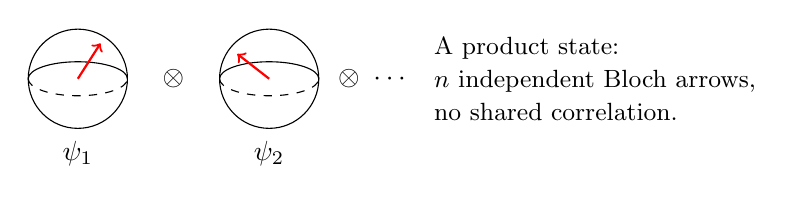
\begin{tikzpicture}[scale=0.9]
  \draw (0,0) circle (0.7);
  \draw[dashed] (-0.7,0) arc (180:360:0.7 and 0.24);
  \draw (0.7,0) arc (0:180:0.7 and 0.24);
  \draw[->,thick,red] (0,0) -- (0.32,0.5);
  \node at (0,-1.05) {$\ket{\psi_1}$};
  \node at (1.35,0) {$\otimes$};
  \begin{scope}[xshift=2.7cm]
    \draw (0,0) circle (0.7);
    \draw[dashed] (-0.7,0) arc (180:360:0.7 and 0.24);
    \draw (0.7,0) arc (0:180:0.7 and 0.24);
    \draw[->,thick,red] (0,0) -- (-0.45,0.35);
    \node at (0,-1.05) {$\ket{\psi_2}$};
  \end{scope}
  \node at (4.15,0) {$\otimes\ \cdots$};
  \node[align=left] at (7.3,0) {\small A product state:\\ \small $n$ independent Bloch arrows,\\ \small no shared correlation.};
\end{tikzpicture}
\end{center}

\subsection{The Bell state and entanglement}
\label{sec:lec01-bell-sub}

\begin{definition}[Bell state]\label{def:lec01-bell}
The \emph{Bell state} (or EPR pair) is the two-qubit state
\begin{equation}
  \ket{\Phi^{+}}=\tfrac{1}{\sqrt2}\bigl(\ket{00}+\ket{11}\bigr).
\end{equation}
\end{definition}

\begin{theorem}[The Bell state is entangled]\label{thm:lec01-bell}
There is no pair of single-qubit states $\ket{\alpha},\ket{\beta}\in\C^{2}$ with
$\ket{\Phi^{+}}=\ket{\alpha}\otimes\ket{\beta}$.
\end{theorem}

\begin{proof}
Suppose for contradiction that such a factorization exists. Write
$\ket{\alpha}=a_0\ket{0}+a_1\ket{1}$ and $\ket{\beta}=b_0\ket{0}+b_1\ket{1}$. Then
\[
  \ket{\alpha}\otimes\ket{\beta}
    =a_0 b_0\ket{00}+a_0 b_1\ket{01}+a_1 b_0\ket{10}+a_1 b_1\ket{11}.
\]
Matching coefficients with
$\ket{\Phi^{+}}=\tfrac{1}{\sqrt2}\ket{00}+0\cdot\ket{01}+0\cdot\ket{10}+\tfrac{1}{\sqrt2}\ket{11}$
requires
\[
  a_0 b_0=\tfrac{1}{\sqrt2},\qquad a_0 b_1=0,\qquad a_1 b_0=0,\qquad a_1 b_1=\tfrac{1}{\sqrt2}.
\]
From $a_0 b_0=\tfrac{1}{\sqrt2}\neq0$ we get $a_0\neq0$ and $b_0\neq0$. Then
$a_0 b_1=0$ forces $b_1=0$, while $a_1 b_0=0$ forces $a_1=0$; hence
$a_1 b_1=0\neq\tfrac{1}{\sqrt2}$, a contradiction. Therefore no factorization exists
and $\ket{\Phi^{+}}$ is entangled.
\end{proof}

\begin{remark}[Physical meaning of entanglement]
The correlations of $\ket{\Phi^{+}}$ have no separable description. Measuring the
first qubit in the computational basis yields $0$ or $1$ with probability $\tfrac12$
each; whatever the outcome, the post-measurement state of the second qubit is forced
to the \emph{same} value ($0\mapsto\ket{0}$, $1\mapsto\ket{1}$). The two outcomes are
perfectly correlated even if the qubits are spatially far apart. This correlation,
inexpressible as any classical mixture of independent single-qubit states, is the
resource behind teleportation, superdense coding, and much of quantum advantage.
\end{remark}

\subsection{Nonlocality and the CHSH inequality}
\label{sec:lec01-chsh}

The correlations of a Bell pair are not merely strong; they are \emph{stronger than
any classical mechanism obeying local realism can produce}. This is the content of
Bell's theorem, which we develop in the sharp form due to Clauser, Horne, Shimony,
and Holt (CHSH). The remarkable point is that a philosophical assumption---that
measurement outcomes are predetermined and unaffected by distant choices---makes a
\emph{quantitative}, testable prediction that quantum mechanics violates.

Two separated parties, Penelope and Odysseus, each receive one qubit of a shared pair. Each
holds a measuring device with two settings. Penelope's two possible measurements return
values $A_1,A_2\in\{+1,-1\}$; Odysseus's return $B_1,B_2\in\{+1,-1\}$. In each run each
party freely picks one setting, so only one of $A_1,A_2$ and one of $B_1,B_2$ is
actually observed. Consider the combination
\begin{equation}\label{eq:lec01-chsh-S}
  S \;=\; A_1B_1-A_1B_2+A_2B_1+A_2B_2 \;=\; A_1(B_1-B_2)+A_2(B_1+B_2).
\end{equation}

\begin{theorem}[CHSH inequality]\label{thm:lec01-chsh}
Suppose the four quantities $A_1,A_2,B_1,B_2\in\{+1,-1\}$ all possess definite values
in every run (\emph{realism}) and that Penelope's values do not depend on Odysseus's setting
or vice versa (\emph{locality}). Then the expectation of $S$ obeys
\[
  \bigl|\,\E[S]\,\bigr|\;=\;\bigl|\,\E[A_1B_1]-\E[A_1B_2]+\E[A_2B_1]+\E[A_2B_2]\,\bigr|\;\le\;2.
\]
\end{theorem}

\begin{proof}
Under realism all four values coexist in each run, so \eqref{eq:lec01-chsh-S} applies
term by term. Since $B_1,B_2\in\{+1,-1\}$, exactly one of $B_1-B_2$ and $B_1+B_2$
is $0$ and the other is $\pm2$. Hence in every run one of the two products
$A_1(B_1-B_2)$, $A_2(B_1+B_2)$ vanishes and the other equals $\pm2$, so $S\in\{+2,-2\}$
deterministically. The average of a quantity that is always $\pm2$ lies in $[-2,2]$,
and linearity of expectation splits $\E[S]$ into the four correlators.
\end{proof}

Quantum mechanics predicts a larger value. Measuring a qubit ``along angle $\theta$''
in the $xz$-plane of the Bloch sphere means measuring the observable with eigenstates
$\ket{\theta}=\cos\tfrac{\theta}{2}\ket{0}+\sin\tfrac{\theta}{2}\ket{1}$ (outcome
$+1$) and its orthogonal partner (outcome $-1$); operationally one applies the
rotation $R_y(-\theta)$ that carries $\ket{\theta}\mapsto\ket{0}$ and then measures in
the computational basis.

\begin{proposition}[Quantum correlator of a Bell pair]\label{prop:lec01-chsh-corr}
If Penelope measures her half of $\ket{\Phi^{+}}=\tfrac{1}{\sqrt2}(\ket{00}+\ket{11})$
along angle $\alpha$ and Odysseus measures his half along angle $\beta$ (with the $\pm1$
labeling above), the correlation of their outcomes is
\begin{equation}\label{eq:lec01-chsh-cosab}
  \E[AB]\;=\;\cos(\alpha-\beta).
\end{equation}
\end{proposition}

\begin{proof}
Applying $R_y(-\alpha)\otimes R_y(-\beta)$ to $\ket{\Phi^{+}}$ and using
$R_y(-\theta)\ket{0}=\cos\tfrac{\theta}{2}\ket{0}-\sin\tfrac{\theta}{2}\ket{1}$,
$R_y(-\theta)\ket{1}=\sin\tfrac{\theta}{2}\ket{0}+\cos\tfrac{\theta}{2}\ket{1}$,
one expands and collects terms. The half-angle addition identities
$\cos\tfrac{\alpha}{2}\cos\tfrac{\beta}{2}+\sin\tfrac{\alpha}{2}\sin\tfrac{\beta}{2}
=\cos\tfrac{\alpha-\beta}{2}$ and
$\sin\tfrac{\alpha}{2}\cos\tfrac{\beta}{2}-\cos\tfrac{\alpha}{2}\sin\tfrac{\beta}{2}
=\sin\tfrac{\alpha-\beta}{2}$ collapse the state to
\[
  \tfrac{1}{\sqrt2}\Bigl(\cos\tfrac{\alpha-\beta}{2}\,\ket{00}
      +\sin\tfrac{\alpha-\beta}{2}\,\ket{01}
      -\sin\tfrac{\alpha-\beta}{2}\,\ket{10}
      +\cos\tfrac{\alpha-\beta}{2}\,\ket{11}\Bigr).
\]
The outcomes $00,11$ (product $+1$) each occur with probability
$\tfrac12\cos^{2}\tfrac{\alpha-\beta}{2}$, and $01,10$ (product $-1$) each with
probability $\tfrac12\sin^{2}\tfrac{\alpha-\beta}{2}$. Hence
$\E[AB]=\cos^{2}\tfrac{\alpha-\beta}{2}-\sin^{2}\tfrac{\alpha-\beta}{2}=\cos(\alpha-\beta)$
by the double-angle identity.
\end{proof}

\begin{corollary}[Tsirelson-point violation]\label{cor:lec01-tsirelson}
With settings $\alpha_1=0,\ \alpha_2=\tfrac{\pi}{2}$ for Penelope and
$\beta_1=\tfrac{\pi}{4},\ \beta_2=\tfrac{3\pi}{4}$ for Odysseus, the quantum prediction is
\[
  \E[S]=\cos(\alpha_1-\beta_1)-\cos(\alpha_1-\beta_2)+\cos(\alpha_2-\beta_1)+\cos(\alpha_2-\beta_2)
       =4\cos\tfrac{\pi}{4}=2\sqrt2\approx2.828,
\]
which exceeds the classical bound $2$ of \cref{thm:lec01-chsh}.
\end{corollary}

\begin{proof}
Each of the four angle differences is $\mp\tfrac{\pi}{4}$: explicitly
$\alpha_1-\beta_1=-\tfrac{\pi}{4}$, $\alpha_1-\beta_2=-\tfrac{3\pi}{4}$,
$\alpha_2-\beta_1=\tfrac{\pi}{4}$, $\alpha_2-\beta_2=-\tfrac{\pi}{4}$. Since
$\cos(\pm\tfrac{\pi}{4})=\tfrac{1}{\sqrt2}$ and $\cos(\tfrac{3\pi}{4})=-\tfrac{1}{\sqrt2}$,
\[
  \E[S]=\tfrac{1}{\sqrt2}-\bigl(-\tfrac{1}{\sqrt2}\bigr)+\tfrac{1}{\sqrt2}+\tfrac{1}{\sqrt2}
       =\tfrac{4}{\sqrt2}=2\sqrt2. \qedhere
\]
\end{proof}

\begin{remark}[What the violation forces us to give up]
The value $2\sqrt2$ is the maximum attainable by any quantum state and measurements
(Tsirelson's bound), and it has been confirmed experimentally---most famously in the
loophole-free tests recognized by the 2022 Nobel Prize in Physics. Because
\cref{thm:lec01-chsh} follows from realism plus locality alone, its experimental
violation means at least one of those assumptions fails: the pre-measurement values
$A_1,A_2,B_1,B_2$ cannot all simultaneously exist as local ``hidden variables.'' The
correlations of $\ket{\Phi^{+}}$ are genuinely nonclassical, yet---as we show next in
\cref{sec:lec01-tele}---they still cannot be used to signal, so no conflict with
relativity arises.
\end{remark}

\section{Gates, universal gate sets, and circuits}
\label{sec:lec01-3}

The postulates of quantum mechanics say that the state of an isolated system evolves
in time by a linear, inner-product-preserving map. On a finite-dimensional Hilbert
space such a map is exactly a unitary operator, and in quantum computing we call it
a gate.

\begin{definition}[Unitary operator / quantum gate]\label{def:lec01-unitary}
Let $\Hilb\cong\C^{d}$ be a finite-dimensional Hilbert space. A linear operator
$U:\Hilb\to\Hilb$ is \emph{unitary} if
\[
  U\dg U = U U\dg = \id,
\]
where $U\dg$ is the conjugate transpose (adjoint) of $U$. A \emph{quantum gate} on
$n$ qubits is a unitary operator on $\Hilb=(\C^{2})^{\otimes n}\cong\C^{2^{n}}$.
\end{definition}

Equivalently, $U$ is unitary iff its columns (or rows) form an orthonormal basis of
$\C^{d}$, iff $U^{-1}=U\dg$. In particular every gate is invertible, so quantum
computation is reversible.

\begin{theorem}[Gates preserve inner products and norm]\label{thm:lec01-unitary-preserves}
Let $U$ be a linear operator on $\Hilb$. The following are equivalent.
\begin{enumerate}[label=\textup{(\roman*)}]
  \item $U$ is unitary, i.e. $U\dg U=\id$.
  \item $U$ preserves inner products: $\braket{U\psi|U\phi}=\braket{\psi|\phi}$ for
        all $\ket{\psi},\ket{\phi}\in\Hilb$.
  \item $U$ preserves norm: $\norm{U\psi}=\norm{\psi}$ for all $\ket{\psi}\in\Hilb$.
\end{enumerate}
\end{theorem}

\begin{proof}
$(\mathrm{i})\Rightarrow(\mathrm{ii})$. Using
$\braket{U\psi|U\phi}=\bra{\psi}U\dg U\ket{\phi}$ and $U\dg U=\id$, we get
$\braket{U\psi|U\phi}=\bra{\psi}\id\ket{\phi}=\braket{\psi|\phi}$.

$(\mathrm{ii})\Rightarrow(\mathrm{iii})$. Take $\ket{\phi}=\ket{\psi}$: then
$\norm{U\psi}^{2}=\braket{U\psi|U\psi}=\braket{\psi|\psi}=\norm{\psi}^{2}$, and
taking nonnegative square roots gives $\norm{U\psi}=\norm{\psi}$.

$(\mathrm{iii})\Rightarrow(\mathrm{i})$. Norm preservation gives
$\bra{\psi}U\dg U\ket{\psi}=\bra{\psi}\id\ket{\psi}$ for all $\ket{\psi}$, so the
self-adjoint operator $M\defeq U\dg U-\id$ satisfies $\bra{\psi}M\ket{\psi}=0$ for
every $\ket{\psi}$. For a self-adjoint operator the quadratic form determines the
operator (via the polarization identity, or by choosing $\ket{\psi}$ to be its
eigenvectors), hence $M=0$, i.e. $U\dg U=\id$. On a finite-dimensional space a left
inverse is a two-sided inverse, so also $UU\dg=\id$ and $U$ is unitary.
\end{proof}

Physically, \cref{thm:lec01-unitary-preserves} says gates map normalized states to
normalized states and never change the ``angle'' between two states; this
inner-product rigidity is exactly what will forbid cloning in \cref{sec:lec01-4}.

\subsection{Single-qubit gates}

\begin{definition}[Pauli, Hadamard, and phase gates]\label{def:lec01-gates}
The \emph{Pauli gates} and identity on $\C^{2}$ are
\[
  I=\begin{pmatrix}1&0\\0&1\end{pmatrix},\quad
  X=\begin{pmatrix}0&1\\1&0\end{pmatrix},\quad
  Y=\begin{pmatrix}0&-\ii\\\ii&0\end{pmatrix},\quad
  Z=\begin{pmatrix}1&0\\0&-1\end{pmatrix}.
\]
The \emph{Hadamard gate} and the \emph{phase gates} $S$ and $T$ are
\[
  H=\frac{1}{\sqrt{2}}\begin{pmatrix}1&1\\1&-1\end{pmatrix},\qquad
  S=\begin{pmatrix}1&0\\0&\ii\end{pmatrix},\qquad
  T=\begin{pmatrix}1&0\\0&\ee^{\ii\pi/4}\end{pmatrix}.
\]
\end{definition}

Each of these is unitary: one checks directly that $X\dg X=Y\dg Y=Z\dg Z=I$, that
$H\dg H=I$, and that $S,T$ are diagonal with unit-modulus entries. In the
computational basis,
\[
  X\ket{0}=\ket{1},\quad X\ket{1}=\ket{0},\qquad
  Z\ket{0}=\ket{0},\quad Z\ket{1}=-\ket{1},
\]
so $X$ is a \emph{bit flip} (the quantum \textsc{not} gate) and $Z$ is a
\emph{phase flip}: it fixes $\ket{0}$ and multiplies $\ket{1}$ by $-1$. The Hadamard
gate creates superpositions,
\[
  H\ket{0}=\ket{+}=\tfrac{1}{\sqrt{2}}(\ket{0}+\ket{1}),\qquad
  H\ket{1}=\ket{-}=\tfrac{1}{\sqrt{2}}(\ket{0}-\ket{1}),
\]
and is self-inverse, $H^{2}=I$. The phase gates leave $\ket{0}$ alone and rotate the
phase of $\ket{1}$: $S$ multiplies it by $\ii$ and $T$ by $\ee^{\ii\pi/4}$.

The four operators $\{I,X,Y,Z\}$ form a basis of the (complex) vector space of
$2\times2$ matrices, so every single-qubit gate is a complex linear combination of
Pauli matrices. Geometrically, a single-qubit pure state corresponds to a point on
the Bloch sphere; the Pauli gates act as rotations by $\pi$ about the $x$, $y$, $z$
axes (up to a global phase). These half-turns are the special cases of a
one-parameter family, which we now work out from the Pauli algebra. For a unit axis
$\hat n\in\R^{3}$ write $\hat n\cdot\vec\sigma\defeq n_xX+n_yY+n_zZ$.

\begin{proposition}[Rotation gates and their Pauli generators]\label{prop:lec01-rot}
The Pauli product identity
$(\vec a\cdot\vec\sigma)(\vec b\cdot\vec\sigma)=(\vec a\cdot\vec b)\,I+\ii(\vec a\times\vec b)\cdot\vec\sigma$
gives $(\hat n\cdot\vec\sigma)^{2}=I$, so the \emph{rotation gate} about $\hat n$ by
angle $\theta$ has the closed form
\[
  R_{\hat n}(\theta)\defeq\exp\!\Big(-\tfrac{\ii\theta}{2}\,\hat n\cdot\vec\sigma\Big)
  =\cos\tfrac{\theta}{2}\,I-\ii\sin\tfrac{\theta}{2}\,(\hat n\cdot\vec\sigma).
\]
With $\hat n=\hat x,\hat y,\hat z$ this yields
\[
  R_x(\theta)=\begin{pmatrix}\cos\tfrac{\theta}{2}&-\ii\sin\tfrac{\theta}{2}\\[2pt]
      -\ii\sin\tfrac{\theta}{2}&\cos\tfrac{\theta}{2}\end{pmatrix},\quad
  R_y(\theta)=\begin{pmatrix}\cos\tfrac{\theta}{2}&-\sin\tfrac{\theta}{2}\\[2pt]
      \sin\tfrac{\theta}{2}&\cos\tfrac{\theta}{2}\end{pmatrix},\quad
  R_z(\theta)=\begin{pmatrix}\ee^{-\ii\theta/2}&0\\0&\ee^{\ii\theta/2}\end{pmatrix},
\]
the gates used for state preparation in \eqref{eq:lec01-rotations}. The Pauli gates
are the half-turns: $X=\ii R_x(\pi)$, $Y=\ii R_y(\pi)$, $Z=\ii R_z(\pi)$.
\end{proposition}

\begin{proof}
Because $(\hat n\cdot\vec\sigma)^{2}=I$, in the series
$\exp(-\ii\alpha\,\hat n\cdot\vec\sigma)=\sum_{k\ge0}\tfrac{(-\ii\alpha)^{k}}{k!}(\hat n\cdot\vec\sigma)^{k}$
(with $\alpha=\theta/2$) the even powers reduce to $I$ and the odd powers to
$\hat n\cdot\vec\sigma$, so they resum to $\cos\alpha\,I-\ii\sin\alpha\,(\hat n\cdot\vec\sigma)$.
Substituting $X,Y,Z$ gives the three matrices; e.g.\
$R_z(\theta)=\cos\tfrac{\theta}{2}I-\ii\sin\tfrac{\theta}{2}Z=\diag(\ee^{-\ii\theta/2},\ee^{\ii\theta/2})$.
Finally $R_z(\pi)=\diag(\ee^{-\ii\pi/2},\ee^{\ii\pi/2})=-\ii Z$, so $Z=\ii R_z(\pi)$,
and likewise for $X,Y$.
\end{proof}

\begin{proposition}[$R_{\hat n}(\theta)$ rotates the Bloch vector]\label{prop:lec01-rodrigues}
Write a single-qubit state as $\rho=\tfrac12(I+\vec r\cdot\vec\sigma)$. Conjugation by
$R_{\hat n}(\theta)$ sends the Bloch vector to its rotation by angle $\theta$ about
$\hat n$:
\[
  R_{\hat n}(\theta)\,\rho\,R_{\hat n}(\theta)\dg=\tfrac12\big(I+\vec r\,'\cdot\vec\sigma\big),
  \quad
  \vec r\,'=\cos\theta\,\vec r+\sin\theta\,(\hat n\times\vec r)+(1-\cos\theta)(\hat n\cdot\vec r)\,\hat n .
\]
\end{proposition}

\begin{proof}
As $R\,I\,R\dg=I$, only the $\vec r\cdot\vec\sigma$ part moves, so it suffices to
conjugate $M\defeq\vec m\cdot\vec\sigma$ for a generic $\vec m$. Put $c=\cos\tfrac{\theta}{2}$,
$s=\sin\tfrac{\theta}{2}$, $N\defeq\hat n\cdot\vec\sigma$, so $R=cI-\ii sN$ and
$R\dg=cI+\ii sN$; then
\[
  RMR\dg=c^{2}M+\ii cs\,[M,N]+s^{2}\,NMN .
\]
The product identity gives $[M,N]=2\ii(\vec m\times\hat n)\cdot\vec\sigma$ and, after a
short computation, $NMN=\big(2(\hat n\cdot\vec m)\,\hat n-\vec m\big)\cdot\vec\sigma$.
Hence $RMR\dg=\vec m\,'\cdot\vec\sigma$ with
\[
  \vec m\,'=c^{2}\vec m+2cs\,(\hat n\times\vec m)+s^{2}\big(2(\hat n\cdot\vec m)\,\hat n-\vec m\big),
\]
and the double-angle identities $c^{2}-s^{2}=\cos\theta$, $2cs=\sin\theta$,
$2s^{2}=1-\cos\theta$ collapse this to Rodrigues' rotation formula. Setting
$\vec m=\vec r$ proves the claim.
\end{proof}

\begin{remark}[Half-angle and the $SU(2)\to SO(3)$ double cover]\label{rem:lec01-doublecover}
The state carries the half-angle $\theta/2$ while the Bloch vector turns by the full
$\theta$. Thus $R_{\hat n}(2\pi)=\cos\pi\,I-\ii\sin\pi\,(\hat n\cdot\vec\sigma)=-I$: a
$2\pi$ Bloch rotation returns the vector but leaves the state with a global phase
$-1$, and only a $4\pi$ turn restores $I$. Equivalently, $R_{\hat n}(\theta)\mapsto
\mathcal R(\hat n,\theta)$ is a two-to-one homomorphism $SU(2)\to SO(3)$, with $\pm
R_{\hat n}(\theta)$ inducing the same (observable) rotation---which is why the Bloch
picture faithfully represents single-qubit gates as ordinary $3$D rotations.
\end{remark}

\begin{lemma}[Hadamard conjugation]\label{lem:lec01-conj}
$H X H = Z$ and $H Z H = X$.
\end{lemma}

\begin{proof}
Recall $H=H\dg$ and $H^{2}=I$. Compute $HXH$ by matrix multiplication. First
\[
  XH=\begin{pmatrix}0&1\\1&0\end{pmatrix}
     \frac{1}{\sqrt2}\begin{pmatrix}1&1\\1&-1\end{pmatrix}
    =\frac{1}{\sqrt2}\begin{pmatrix}1&-1\\1&1\end{pmatrix},
\]
and then
\[
  HXH=\frac{1}{\sqrt2}\begin{pmatrix}1&1\\1&-1\end{pmatrix}\cdot
      \frac{1}{\sqrt2}\begin{pmatrix}1&-1\\1&1\end{pmatrix}
     =\frac{1}{2}\begin{pmatrix}2&0\\0&-2\end{pmatrix}
     =\begin{pmatrix}1&0\\0&-1\end{pmatrix}=Z.
\]
For the second identity, conjugate the first by $H$ on both sides and use $H^{2}=I$:
from $HXH=Z$ we get $H(HXH)H=HZH$, i.e. $(H^{2})X(H^{2})=HZH$, so $X=HZH$.
\end{proof}

\Cref{lem:lec01-conj} is the precise statement that $H$ is a ``bridge'' between the
bit-flip and phase-flip pictures: a phase flip in the computational basis looks like
a bit flip in the Hadamard ($\ket{+},\ket{-}$) basis, and vice versa. Two further
identities are recorded for reference.

\begin{proposition}\label{prop:lec01-yxz}
$Y=\ii XZ$ and $S=T^{2}$.
\end{proposition}

\begin{proof}
Direct computation:
\[
  XZ=\begin{pmatrix}0&1\\1&0\end{pmatrix}
     \begin{pmatrix}1&0\\0&-1\end{pmatrix}
    =\begin{pmatrix}0&-1\\1&0\end{pmatrix},\qquad
  \ii XZ=\begin{pmatrix}0&-\ii\\\ii&0\end{pmatrix}=Y.
\]
For the phase gates, $T$ is diagonal so $T^{2}=\diag(1,\ee^{\ii\pi/4})^{2}=\diag(1,\ee^{\ii\pi/2})=\diag(1,\ii)=S$.
\end{proof}

\begin{remark}[$T$ is non-Clifford]
The \emph{Clifford group} is generated by $\{H,S,\CNOT\}$ (equivalently, the
unitaries that map the Pauli group to itself under conjugation). The identities above
show $X,Y,Z$ and $S=T^{2}$ lie in this group. The $T$ gate does \emph{not}:
conjugating a Pauli by $T$ produces a superposition of Paulis rather than another
Pauli. This matters because the Gottesman--Knill theorem says Clifford circuits are
efficiently classically simulable; the $T$ gate is precisely the ingredient that
lifts a gate set to universality for quantum computation.
\end{remark}

\subsection{Multi-qubit gates}

To act on more than one qubit we take tensor products. A gate $A$ on qubit~$0$ and
$B$ on qubit~$1$ acts on the joint state as $A\otimes B$, with
$(A\otimes B)(\ket{u}\otimes\ket{v})=A\ket{u}\otimes B\ket{v}$. The most important
genuinely two-qubit gate is the controlled-\textsc{not}.

\begin{definition}[$\CNOT$ and Toffoli]\label{def:lec01-cnot}
The \emph{controlled-\textsc{not}} gate $\CNOT$ acts on two qubits (control $a$,
target $b$) by
\[
  \CNOT\ket{a,b}=\ket{a,\,a\oplus b},\qquad a,b\in\{0,1\},
\]
where $\oplus$ is addition modulo $2$. In the ordered computational basis
$\ket{00},\ket{01},\ket{10},\ket{11}$ its matrix is the $4\times4$ permutation
unitary
\[
  \CNOT=\begin{pmatrix}
    1&0&0&0\\ 0&1&0&0\\ 0&0&0&1\\ 0&0&1&0
  \end{pmatrix}.
\]
The \emph{Toffoli} (or \textsc{ccnot}) gate acts on three qubits by
$\mathrm{CCNOT}\ket{a,b,c}=\ket{a,\,b,\,(a\wedge b)\oplus c}$, flipping the target
$c$ exactly when both controls $a,b$ equal $1$.
\end{definition}

Since $\CNOT$ permutes the four basis vectors it is a permutation matrix, hence
unitary; the same holds for the Toffoli gate, which swaps
$\ket{110}\leftrightarrow\ket{111}$. Both are their own inverse. The Toffoli gate is
universal for classical reversible computation: with ancillas it can implement
\textsc{and}, \textsc{not}, and fan-out, so any Boolean circuit can be made
reversible.

\begin{remark}[Why XOR keeps oracles reversible]
A classical oracle for $f:\{0,1\}^{n}\to\{0,1\}$ is realized quantumly as
$\Uf\ket{x}\ket{b}=\ket{x}\ket{b\oplus f(x)}$. Writing the answer with $\oplus$ rather
than overwriting $b$ with $f(x)$ is what makes $\Uf$ a permutation of basis states,
hence unitary and reversible: applying $\Uf$ twice returns $\ket{b\oplus f(x)\oplus f(x)}=\ket{b}$,
so $\Uf^{2}=\id$. A plain overwrite $b\mapsto f(x)$ is generally not injective and
cannot be unitary. The $\CNOT$ rule $b\mapsto a\oplus b$ is the single-bit instance
of this construction.
\end{remark}

\subsection{Reading quantum circuits}

A \emph{quantum circuit} is a diagram in which each horizontal wire is a qubit and
gates are drawn on the wires. Three conventions govern how to read one.
\begin{enumerate}[label=(\arabic*)]
  \item \textbf{Time flows left to right.} The input state sits at the far left; a
        gate drawn further left is applied earlier.
  \item \textbf{Controls.} On a controlled gate, a filled dot $\bullet$ marks a
        control that activates when the qubit is $\ket{1}$; an open dot $\circ$
        marks a $0$-control, which activates when the qubit is $\ket{0}$.
  \item \textbf{Matrix order is reversed.} If the circuit applies $U_{1}$ first, then
        $U_{2}$, the overall unitary is the \emph{reverse-order} product $U=U_{2}\,U_{1}$,
        because operators act on the ket to their right. For a length-$m$ sequence,
        $U=U_{m}U_{m-1}\cdots U_{1}$.
\end{enumerate}

A controlled-$U$ gate with control $a$ can be written compactly as
$c\text{-}U\,\ket{a}\ket{b}=\ket{a}\,U^{a}\ket{b}$, so $U$ is applied to the target
raised to the power $a\in\{0,1\}$ (nothing happens when $a=0$). The \textsc{swap}
gate exchanges two qubits, $\mathrm{SWAP}\ket{a,b}=\ket{b,a}$; it can be built from
three $\CNOT$s.

\begin{definition}[Circuit depth]\label{def:lec01-depth}
Group the gates of a circuit into \emph{layers}, where a layer is a maximal set of
gates acting on disjoint qubits that can be executed simultaneously. The \emph{depth}
of the circuit is the number of layers, equivalently the largest number of gates on
any single input-to-output path through the diagram.
\end{definition}

Gates acting on disjoint sets of qubits commute as tensor factors and run in
parallel, so depth (not total gate count) measures wall-clock runtime, and keeping
depth low is central to running on noisy hardware.

\begin{example}[A small circuit's unitary as a reverse-order product]
Consider one qubit with, from left to right, an $H$ gate, then an $S$ gate, then
another $H$ gate. The overall unitary is the reverse-order product
\[
  U = H\,S\,H
    = \frac{1}{2}\begin{pmatrix}1&1\\1&-1\end{pmatrix}
      \begin{pmatrix}1&0\\0&\ii\end{pmatrix}
      \begin{pmatrix}1&1\\1&-1\end{pmatrix}
    = \frac{1}{2}\begin{pmatrix}1+\ii&1-\ii\\1-\ii&1+\ii\end{pmatrix}.
\]
One checks $U\dg U=I$, confirming the composite is again a gate.
\end{example}

\subsection{Building a Bell state}

We now assemble single- and two-qubit gates into a circuit that creates entanglement.
Prepare two qubits in $\ket{00}$, apply $H$ to qubit~$0$, then apply $\CNOT$ with
qubit~$0$ as control and qubit~$1$ as target.

\begin{theorem}[Bell-state preparation]\label{thm:lec01-bellprep}
With qubit~$0$ the control and qubit~$1$ the target,
\[
  \CNOT\,(H\otimes I)\,\ket{00}
    = \tfrac{1}{\sqrt2}\big(\ket{00}+\ket{11}\big)=\ket{\Phi^{+}}.
\]
\end{theorem}

\begin{proof}
First apply $H\otimes I$. Since $H\ket{0}=\tfrac{1}{\sqrt2}(\ket{0}+\ket{1})$ and
$I\ket{0}=\ket{0}$,
\[
  (H\otimes I)\ket{00}
    = \tfrac{1}{\sqrt2}(\ket{0}+\ket{1})\otimes\ket{0}
    = \tfrac{1}{\sqrt2}\big(\ket{00}+\ket{10}\big).
\]
Now apply $\CNOT$ term by term using $\CNOT\ket{a,b}=\ket{a,a\oplus b}$. On $\ket{00}$
the control is $0$, so the state is unchanged. On $\ket{10}$ the control is $1$, so
the target flips: $\ket{10}\mapsto\ket{11}$. Hence
\[
  \CNOT\,\tfrac{1}{\sqrt2}\big(\ket{00}+\ket{10}\big)
    = \tfrac{1}{\sqrt2}\big(\ket{00}+\ket{11}\big)=\ket{\Phi^{+}}. \qedhere
\]
\end{proof}

By \cref{thm:lec01-bell} the state $\ket{\Phi^{+}}$ is entangled, so this two-gate
circuit turns a product input into a maximally entangled Bell pair.

\subsection{Universal gate sets and compilation}

\begin{definition}[Universal gate set]\label{def:lec01-universal}
A finite set $\mathcal{G}$ of gates is \emph{universal} if the unitaries generated by
applying gates from $\mathcal{G}$ to arbitrary subsets of qubits are dense in the
group of all $n$-qubit unitaries (up to global phase): for every target unitary $U$
and every $\varepsilon>0$ there is a finite circuit $V$ over $\mathcal{G}$ with
$\norm{U-V}\le\varepsilon$.
\end{definition}

Two facts underlie this definition. First, any $n$-qubit unitary can be written
\emph{exactly} as a product of single-qubit and two-qubit gates,
$U=U_{m}U_{m-1}\cdots U_{1}$, though $m$ may be exponential in $n$. Second, a fixed
\emph{finite} set already suffices to approximate every gate: the set
$\mathcal{G}=\{H,\,T,\,\CNOT\}$ is universal. We settle for approximation because a
discrete set cannot hit a continuum of unitaries exactly, but it can come within any
$\varepsilon$.

\begin{remark}[Solovay--Kitaev cost]
The Solovay--Kitaev theorem quantifies the price of this discretization: any
single-qubit gate can be approximated to error $\varepsilon$ by a circuit of
$\bigo\!\big(\polylog(1/\varepsilon)\big)$ gates from a universal set, and an
$m$-gate circuit can be recompiled into the finite set using only
$\bigo\!\big(m\,\polylog(m/\varepsilon)\big)$ gates, found by an efficient classical
algorithm. The overhead is thus only polylogarithmic in the inverse precision, which
is why compiling ideal circuits to a fixed hardware gate set is practical.
\end{remark}

\begin{remark}[Why Solovay--Kitaev works (sketch)]\label{rem:lec01-sk-sketch}
The polylogarithmic bound comes from a recursion that sharpens an approximation by
representing its \emph{error} with ever-smaller gates. Assume $\mathcal{G}$ is closed
under inverses.
\emph{(i) Base net.} Density of $\langle\mathcal{G}\rangle$ together with compactness of
$SU(2)$ gives a fixed accuracy $\varepsilon_0$ reachable by \emph{every} gate using
words of bounded length.
\emph{(ii) Commutator lemma.} Any $\Delta$ near the identity, $\norm{\Delta-\id}\le\delta$,
factors as a group commutator $\Delta=VWV\dg W\dg$ up to $\bigo(\delta^{3/2})$, where
$V,W$ are only $\bigo(\sqrt{\delta})$ from the identity---writing
$V=\ee^{-\ii A}$, $W=\ee^{-\ii B}$ with $A,B=\bigo(\sqrt{\delta})$, one has
$VWV\dg W\dg=\ee^{-[A,B]+\bigo(\delta^{3/2})}$ and $[A,B]=\bigo(\delta)$.
\emph{(iii) Recursion.} Given a level-$(n{-}1)$ approximation $U_{n-1}$ of accuracy
$\varepsilon_{n-1}$, decompose the residual $\Delta=U\,U_{n-1}\dg$ by the lemma,
approximate $V,W$ at level $n{-}1$, and glue the commutator onto $U_{n-1}$:
\[
  \varepsilon_n=\bigo\!\big(\varepsilon_{n-1}^{3/2}\big),\qquad
  \ell_n=5\,\ell_{n-1}+\bigo(1).
\]
The exponent $3/2$ makes the error fall doubly exponentially, so
$n=\bigo(\log\log(1/\varepsilon))$ levels suffice; unrolling $\ell_n=5^{n}\ell_0$ then
gives $\ell(\varepsilon)=\bigo\!\big((\log(1/\varepsilon))^{\log 5/\log(3/2)}\big)$,
with exponent $\approx 3.97$. A single-qubit rotation is just the generic target
$U\in SU(2)$, so the bound applies to it directly (Dawson \& Nielsen,
\emph{The Solovay--Kitaev algorithm}, Quantum Inf.\ Comput.\ \textbf{6} (2006) 81).
\end{remark}

Running an abstract circuit on a real device requires \emph{compilation}:
(i) rewriting logical gates such as $H$, $T$, $\CNOT$ into the machine's native gate
set; and (ii) inserting \textsc{swap} gates to route qubits, because hardware qubits
are not all pairwise connected. Throughout one minimizes gate count and depth to
suppress noise and maximize fidelity.

\subsection{Worked example: a reversible binary adder}
\label{sec:lec01-adder}

The computational basis of $n$ qubits is labeled by the integers
$0,1,\dots,2^{n}-1$: we identify the string $\ket{k_1\cdots k_n}$ with its
base-two value $k=\sum_{l=1}^{n}k_l\,2^{\,n-l}$, so that $\ket{10}=\ket{2}$,
$\ket{11}=\ket{3}$, and a three-qubit register ranges over $\ket{0},\dots,\ket{7}$.
A circuit that permutes these basis states therefore \emph{computes an
integer-valued function}, and the final computational-basis measurement returns
the answer as an ordinary number. We make this concrete by building a circuit
that adds two-bit numbers, which at the same time demonstrates the claim
following \cref{def:lec01-cnot} that the Toffoli gate is universal for classical
reversible computation. Here $\oplus$ is addition modulo~$2$ (the \textsc{xor},
computed by $\CNOT$) and $\wedge$ is the logical \textsc{and} (computed by a
Toffoli onto a $\ket{0}$ ancilla).

To add $A_1A_0$ and $B_1B_0$ we work column by column, exactly as in grade-school
addition but in base two. The rightmost column produces a sum bit $S_0$ and a
carry $C_1$; the next column adds $A_1$, $B_1$, and the incoming carry $C_1$ to
produce $S_1$ and a final carry $C_2$; and the result is the three-bit number
$C_2S_1S_0$ (for example, $2+3$ is $10+11=101=5$). In the familiar columnar layout,
with each carry written above the column it feeds:
\[
\begin{array}{r@{\;}c@{\;}c@{\;}c}
    & C_2 & C_1 &     \\
    &     & A_1 & A_0 \\
  + &     & B_1 & B_0 \\ \hline
    & C_2 & S_1 & S_0
\end{array}
\qquad\text{e.g.}\qquad
\begin{array}{r@{\;}c@{\;}c@{\;}c}
    & 1 & 0 &   \\
    &   & 1 & 0 \\
  + &   & 1 & 1 \\ \hline
    & 1 & 0 & 1
\end{array}
\]

\paragraph{Half adder.} The rightmost column has no incoming carry, so
\[
  S_0=A_0\oplus B_0,\qquad C_1=A_0\wedge B_0,
\]
as the truth table confirms:
\begin{center}
\begin{tabular}{cc@{\qquad}cc}
\toprule
$A_0$ & $B_0$ & $C_1$ & $S_0$\\ \midrule
0 & 0 & 0 & 0\\
0 & 1 & 0 & 1\\
1 & 0 & 0 & 1\\
1 & 1 & 1 & 0\\ \bottomrule
\end{tabular}
\end{center}
The sum bit is a single $\CNOT$ (control $A_0$, target $B_0$), and the carry is a
Toffoli (controls $A_0,B_0$) writing $A_0\wedge B_0$ onto a fresh $\ket{0}$
ancilla. Because the $\CNOT$ overwrites $B_0$, we compute the carry \emph{first}:
\begin{center}
\begin{quantikz}
\lstick{$\ket{A_0}$} & \ctrl{1} & \ctrl{1} & \qw \\
\lstick{$\ket{B_0}$} & \ctrl{1} & \targ{}  & \qw \\
\lstick{$\ket{0}$}   & \targ{}  & \qw      & \qw
\end{quantikz}
\end{center}
Reading top to bottom, the output wires hold $A_0$, the sum $S_0=A_0\oplus B_0$,
and the carry $C_1=A_0\wedge B_0$.

\paragraph{Full adder.} The next column sums three bits, $C_1$, $A_1$, $B_1$:
\[
  S_1=C_1\oplus A_1\oplus B_1,\qquad
  C_2=(A_1\wedge B_1)\oplus(C_1\wedge A_1)\oplus(C_1\wedge B_1).
\]
These rules are confirmed by the truth table over the three input bits $C_1,A_1,B_1$:
\begin{center}
\begin{tabular}{ccc@{\qquad}cc}
\toprule
$C_1$ & $A_1$ & $B_1$ & $C_2$ & $S_1$\\ \midrule
0 & 0 & 0 & 0 & 0\\
0 & 0 & 1 & 0 & 1\\
0 & 1 & 0 & 0 & 1\\
0 & 1 & 1 & 1 & 0\\
1 & 0 & 0 & 0 & 1\\
1 & 0 & 1 & 1 & 0\\
1 & 1 & 0 & 1 & 0\\
1 & 1 & 1 & 1 & 1\\ \bottomrule
\end{tabular}
\end{center}
The carry $C_2$ is accumulated onto a $\ket{0}$ ancilla by three Toffolis, one for
each product; the sum $S_1$ is then two $\CNOT$s targeting the $B_1$ wire (controls
$C_1$ and $A_1$). As before we compute the carry first, since forming $S_1$
overwrites $B_1$:
\begin{center}
\begin{quantikz}
\lstick{$\ket{C_1}$} & \qw      & \ctrl{3} & \ctrl{3} & \ctrl{2} & \qw      & \qw\\
\lstick{$\ket{A_1}$} & \ctrl{2} & \ctrl{2} & \qw      & \qw      & \ctrl{1} & \qw\\
\lstick{$\ket{B_1}$} & \ctrl{1} & \qw      & \ctrl{1} & \targ{}  & \targ{}  & \qw\\
\lstick{$\ket{0}$}   & \targ{}  & \targ{}  & \targ{}  & \qw      & \qw      & \qw
\end{quantikz}
\end{center}
The output wires now hold $C_1$, $A_1$, the sum $S_1$, and the carry $C_2$ on the
ancilla.

\paragraph{The two-bit adder.} Cascading the two blocks---the half adder's carry
output $C_1$ feeds the full adder---gives the complete circuit for
$A_1A_0+B_1B_0$: the half adder produces $S_0$ and $C_1$ from $A_0,B_0$, and the
full adder consumes $C_1,A_1,B_1$ to produce $S_1$ and $C_2$. Measuring the three
wires that hold $S_0$, $S_1$, $C_2$ returns the binary digits of the sum. For
instance, to compute $3+3$ one sets $A_1A_0=B_1B_0=11$ by applying $X$ to the four
input qubits (initialized to $\ket{0}$) and reads the output $110_2=6$. The complete
circuit is drawn in \cref{fig:lec01-adder2}.

\begin{figure}[htbp]
\centering
\begin{quantikz}
\lstick{$\ket{A_0}$} & \ctrl{1} & \ctrl{1} & \qw      & \qw      & \qw      & \qw      & \qw      & \qw \\
\lstick{$\ket{B_0}$} & \ctrl{1} & \targ{}  & \qw      & \qw      & \qw      & \qw      & \qw      & \qw \\
\lstick{$\ket{0}$}   & \targ{}  & \qw      & \qw      & \ctrl{3} & \ctrl{3} & \ctrl{1} & \qw      & \qw \\
\lstick{$\ket{A_1}$} & \qw      & \qw      & \ctrl{1} & \ctrl{2} & \qw      & \targ{}  & \ctrl{1} & \qw \\
\lstick{$\ket{B_1}$} & \qw      & \qw      & \ctrl{1} & \qw      & \ctrl{1} & \qw      & \targ{}  & \qw \\
\lstick{$\ket{0}$}   & \qw      & \qw      & \targ{}  & \targ{}  & \targ{}  & \qw      & \qw      & \qw
\end{quantikz}
\caption{The two-bit ripple adder $A_1A_0+B_1B_0\mapsto C_2S_1S_0$: the half adder
(first two gates) computes $S_0,C_1$, and the cascaded full adder computes $S_1,C_2$
(three Toffolis for the carry, then two $\CNOT$s for the sum). Output wires, top to
bottom: $A_0$, $S_0$, $C_1$, $C_1\oplus A_1$, $S_1$, $C_2$; the sum is $C_2S_1S_0$.
After Brody, Fig.~7.12.}
\label{fig:lec01-adder2}
\end{figure}

\paragraph{Running the adder.} On hardware every qubit starts in $\ket{0}$, so an
input bit is set to $1$ by a leading $X$ (\textsc{not}) gate placed before the adder.
\Cref{fig:lec01-adder-runs} shows three cases: $0+0$ (no $X$ gates), $1+1=01+01$
($X$ on $A_0$ and $B_0$), and $1+2=01+10$ ($X$ on $A_0$ and $B_1$); measuring
$S_0,S_1,C_2$ then reads $000_2=0$, $010_2=2$, and $011_2=3$ respectively.

\begin{figure}[htbp]
\centering
\begin{tabular}{c}
$0+0$\\[3pt]
\begin{quantikz}
\lstick{$\ket{0}$} & \qw      & \gate[6]{\text{2-bit adder}} & \qw \\
\lstick{$\ket{0}$} & \qw      &                              & \meter{} \\
\lstick{$\ket{0}$} & \qw      &                              & \qw \\
\lstick{$\ket{0}$} & \qw      &                              & \qw \\
\lstick{$\ket{0}$} & \qw      &                              & \meter{} \\
\lstick{$\ket{0}$} & \qw      &                              & \meter{}
\end{quantikz}\\[14pt]
$1+1=01+01$\\[3pt]
\begin{quantikz}
\lstick{$\ket{0}$} & \gate{X} & \gate[6]{\text{2-bit adder}} & \qw \\
\lstick{$\ket{0}$} & \gate{X} &                              & \meter{} \\
\lstick{$\ket{0}$} & \qw      &                              & \qw \\
\lstick{$\ket{0}$} & \qw      &                              & \qw \\
\lstick{$\ket{0}$} & \qw      &                              & \meter{} \\
\lstick{$\ket{0}$} & \qw      &                              & \meter{}
\end{quantikz}\\[14pt]
$1+2=01+10$\\[3pt]
\begin{quantikz}
\lstick{$\ket{0}$} & \gate{X} & \gate[6]{\text{2-bit adder}} & \qw \\
\lstick{$\ket{0}$} & \qw      &                              & \meter{} \\
\lstick{$\ket{0}$} & \qw      &                              & \qw \\
\lstick{$\ket{0}$} & \qw      &                              & \qw \\
\lstick{$\ket{0}$} & \gate{X} &                              & \meter{} \\
\lstick{$\ket{0}$} & \qw      &                              & \meter{}
\end{quantikz}
\end{tabular}
\caption{The adder of \cref{fig:lec01-adder2} configured for three inputs (the box
hides its internal gates): leading $X$ gates load the operands and the three meters
read $S_0,S_1,C_2$. Top to bottom the wires are $A_0,B_0,\ket{0},A_1,B_1,\ket{0}$.
After Brody, Figs.~7.13, 7.15, and 7.17.}
\label{fig:lec01-adder-runs}
\end{figure}

\begin{remark}[Reversibility, ancillas, and garbage]
Every gate above is a permutation of basis states, so the adder is one large
permutation unitary---reversible, exactly as \cref{thm:lec01-unitary-preserves}
requires of any gate. Reversibility is bought with bookkeeping: results are
written with $\oplus$ onto fresh $\ket{0}$ ancillas rather than overwriting inputs,
so the circuit also carries along the original inputs and some intermediate
``garbage.'' Bennett's trick---copy the final answer out with $\CNOT$s, then run
the circuit backward---uncomputes the garbage and resets the ancillas to
$\ket{0}$, which is what lets an adder serve as a clean subroutine inside a larger
coherent algorithm. Finally, the many Toffoli gates make the adder demanding on
real hardware, where gate errors accumulate with circuit size; this is an early
hint of why controlling noise becomes central as circuits grow.
\end{remark}

\section{State preparation and measurement}
\label{sec:lec01-prepmeas}

Every quantum algorithm is bracketed by two operations that are not gates: it must
begin by \emph{preparing} an input state and end by \emph{measuring} an output. The
gate model of \cref{sec:lec01-3} describes the unitary evolution in between; this
section treats the two endpoints systematically, building on the computational-basis
Born rule already stated in \cref{sec:lec01-1}. Both endpoints have a cost, and that
cost often dominates: a beautiful $\poly(n)$-gate circuit is useless if loading its
input takes $\bigo(2^{n})$ gates, and an expectation value is only as good as the
number of measurement repetitions one can afford.

\subsection{Preparing states from \texorpdfstring{$\ket{0\cdots0}$}{|0...0>}}

By convention every register starts in the all-zeros state $\ket{0}^{\otimes n}=\ket{0\cdots0}$.
Preparing a target state means finding a circuit that maps $\ket{0\cdots0}$ to it.

\begin{proposition}[Basis states and the uniform superposition]\label{prop:lec01-prepbasic}
Let $x=x_{1}\cdots x_{n}\in\{0,1\}^{n}$.
\begin{enumerate}[label=\textup{(\alph*)}]
  \item The computational basis state $\ket{x}$ is prepared from $\ket{0\cdots0}$ by
        applying $X$ to each qubit $j$ with $x_{j}=1$; that is,
        $\bigl(\bigotimes_{j}X^{x_{j}}\bigr)\ket{0\cdots0}=\ket{x}$, using at most
        $n$ gates.
  \item The uniform superposition over all $2^{n}$ strings is prepared by one
        Hadamard per qubit,
        \begin{equation}\label{eq:lec01-uniform}
          H^{\otimes n}\ket{0\cdots0}
            =\frac{1}{\sqrt{2^{n}}}\sum_{x\in\{0,1\}^{n}}\ket{x},
        \end{equation}
        using exactly $n$ gates.
\end{enumerate}
\end{proposition}

\begin{proof}
(a) $X^{x_{j}}\ket{0}=\ket{x_{j}}$ acts qubitwise, and the tensor product of the
single-qubit results is $\ket{x_{1}}\cdots\ket{x_{n}}=\ket{x}$.
(b) On one qubit $H\ket{0}=\tfrac{1}{\sqrt2}(\ket{0}+\ket{1})$. Taking the tensor
power and expanding the product of $n$ sums,
\[
  H^{\otimes n}\ket{0\cdots0}
    =\bigotimes_{j=1}^{n}\tfrac{1}{\sqrt2}(\ket{0}+\ket{1})
    =\frac{1}{\sqrt{2^{n}}}\sum_{x\in\{0,1\}^{n}}\ket{x},
\]
since choosing $\ket{0}$ or $\ket{1}$ from each factor enumerates all bit strings $x$
exactly once.
\end{proof}

The uniform superposition \eqref{eq:lec01-uniform} is the workhorse input of the
query algorithms of Part~I: a single depth-one layer of Hadamards places the register
in an equal-weight combination of all $2^{n}$ inputs, on which an oracle can then act
``in parallel.''

\subsection{Single-qubit state synthesis}

A general single-qubit target is, up to global phase, the Bloch state
$\ket{\psi(\theta,\varphi)}=\cos\tfrac{\theta}{2}\ket{0}+\ee^{\ii\varphi}\sin\tfrac{\theta}{2}\ket{1}$
of \cref{prop:lec01-bloch}. It is reached from $\ket{0}$ by a rotation about the $y$
axis followed by one about the $z$ axis, where the rotation gates are
\begin{equation}\label{eq:lec01-rotations}
  R_{y}(\theta)=\ee^{-\ii\theta Y/2}
    =\begin{pmatrix}\cos\tfrac{\theta}{2}&-\sin\tfrac{\theta}{2}\\[2pt]
      \sin\tfrac{\theta}{2}&\phantom{-}\cos\tfrac{\theta}{2}\end{pmatrix},
  \qquad
  R_{z}(\varphi)=\ee^{-\ii\varphi Z/2}
    =\begin{pmatrix}\ee^{-\ii\varphi/2}&0\\ 0&\ee^{\ii\varphi/2}\end{pmatrix}.
\end{equation}

\begin{proposition}[Single-qubit preparation]\label{prop:lec01-1qprep}
For any $\theta\in[0,\pi]$ and $\varphi\in[0,2\pi)$,
\[
  R_{z}(\varphi)\,R_{y}(\theta)\,\ket{0}
    =\ee^{-\ii\varphi/2}\Bigl(\cos\tfrac{\theta}{2}\ket{0}+\ee^{\ii\varphi}\sin\tfrac{\theta}{2}\ket{1}\Bigr),
\]
so up to the global phase $\ee^{-\ii\varphi/2}$ the circuit prepares
$\ket{\psi(\theta,\varphi)}$ with two gates.
\end{proposition}

\begin{proof}
From \eqref{eq:lec01-rotations},
$R_{y}(\theta)\ket{0}=\cos\tfrac{\theta}{2}\ket{0}+\sin\tfrac{\theta}{2}\ket{1}$.
Applying the diagonal $R_{z}(\varphi)$ multiplies the $\ket{0}$ amplitude by
$\ee^{-\ii\varphi/2}$ and the $\ket{1}$ amplitude by $\ee^{\ii\varphi/2}$:
\[
  R_{z}(\varphi)R_{y}(\theta)\ket{0}
    =\ee^{-\ii\varphi/2}\cos\tfrac{\theta}{2}\ket{0}
     +\ee^{\ii\varphi/2}\sin\tfrac{\theta}{2}\ket{1}
    =\ee^{-\ii\varphi/2}\Bigl(\cos\tfrac{\theta}{2}\ket{0}+\ee^{\ii\varphi}\sin\tfrac{\theta}{2}\ket{1}\Bigr).
\]
The overall factor $\ee^{-\ii\varphi/2}$ is an unobservable global phase
(\cref{rem:lec01-global}).
\end{proof}

\begin{example}[Preparing $\ket{+\ii}$]\label{exa:lec01-prepplusi}
The state $\ket{+\ii}=\tfrac{1}{\sqrt2}(\ket{0}+\ii\ket{1})$ has Bloch angles
$\theta=\pi/2$ (equal moduli) and $\varphi=\pi/2$ (relative phase $\ii=\ee^{\ii\pi/2}$).
By \cref{prop:lec01-1qprep} it is prepared by $R_{z}(\pi/2)R_{y}(\pi/2)\ket{0}$: the
$R_{y}(\pi/2)$ produces $\ket{+}=\tfrac{1}{\sqrt2}(\ket{0}+\ket{1})$, and
$R_{z}(\pi/2)$ then multiplies the $\ket{1}$ amplitude by $\ee^{\ii\pi/2}=\ii$
relative to the $\ket{0}$ amplitude, giving $\tfrac{1}{\sqrt2}(\ket{0}+\ii\ket{1})$ up
to global phase. Note $S\ket{+}=\ket{+\ii}$ as well, so a single $S$ gate achieves the
same result here.
\end{example}

\subsection{General amplitude encoding}

Preparing an arbitrary $n$-qubit state $\ket{\psi}=\sum_{x\in\{0,1\}^{n}}a_{x}\ket{x}$
from a classical list of the $2^{n}$ amplitudes $\{a_{x}\}$ is far more expensive than
the special cases above.

\begin{theorem}[Cost of exact amplitude encoding]\label{thm:lec01-prepcost}
Every $n$-qubit pure state $\ket{\psi}=\sum_{x}a_{x}\ket{x}$ can be prepared exactly
from $\ket{0\cdots0}$ by a circuit of single-qubit rotations and $\CNOT$ gates, and
$\bigo(2^{n})$ gates suffice. Conversely, a counting argument shows that
$\Omega(2^{n})$ gates are necessary for generic states, so this scaling is optimal up
to constants.
\end{theorem}

We state the result at this level and do not reproduce the construction; the standard
recipe of Möttönen, Vartiainen, Bergholm, and Salomaa, and the equivalent
Shende--Bullock--Markov decomposition, prepare $\ket{\psi}$ by a cascade of
uniformly controlled $R_{y}$ and $R_{z}$ rotations, one layer per qubit, encoding the
amplitudes' moduli and phases in the rotation angles. The upper bound matches an
information-theoretic lower bound: specifying a generic unit vector in $\C^{2^{n}}$
requires $\sim 2^{n}$ real parameters, and each gate supplies only $\bigo(1)$, so no
subexponential circuit can reach all states.

\begin{remark}[Efficient special cases]\label{rem:lec01-prepefficient}
The exponential cost of \cref{thm:lec01-prepcost} is a worst case over \emph{all}
states; the states that arise in practice are usually structured, and structure buys
efficiency.
\begin{itemize}[nosep]
  \item \emph{Product states} $\ket{\psi_{1}}\otimes\cdots\otimes\ket{\psi_{n}}$ cost
        $\bigo(n)$ gates: prepare each qubit independently by \cref{prop:lec01-1qprep}.
  \item \emph{Efficiently computable amplitudes.} If the $a_{x}$ are given by a
        formula one can evaluate reversibly (for example a discretized smooth density,
        via the Grover--Rudolph procedure that recursively rotates on conditional
        probabilities), the state can be prepared in $\poly(n)$ gates.
  \item \emph{Sparse states} with only $s$ nonzero amplitudes can be prepared in
        $\bigo(s\,n)$ gates, independent of the full dimension $2^{n}$.
\end{itemize}
When the amplitudes come from external data rather than a formula, one instead posits
a black-box \emph{state-preparation oracle}; this input model, and its role in
quantum numerical linear algebra, is developed in \cref{ch:lec06}.
\end{remark}

\subsection{Projective measurement}

The computational-basis Born rule of \cref{sec:lec01-1} is the special case of a more
general measurement postulate, which we now state in full.

\begin{definition}[Projective (von Neumann) measurement]\label{def:lec01-projmeas}
An \emph{observable} is a Hermitian operator $O=O\dg$ on $\Hilb$. Writing its spectral
decomposition as $O=\sum_{m}m\,P_{m}$, where the distinct real eigenvalues $m$ index
mutually orthogonal projectors $P_{m}$ (so $P_{m}P_{m'}=\delta_{mm'}P_{m}$,
$P_{m}\dg=P_{m}$) that resolve the identity, $\sum_{m}P_{m}=\id$, the associated
\emph{projective measurement} of a state $\ket{\psi}$ returns outcome $m$ with
probability
\begin{equation}\label{eq:lec01-projprob}
  p_{m}=\bra{\psi}P_{m}\ket{\psi}=\norm{P_{m}\ket{\psi}}^{2},
\end{equation}
and leaves the post-measurement state
\begin{equation}\label{eq:lec01-projpost}
  \frac{P_{m}\ket{\psi}}{\sqrt{p_{m}}}\qquad(\text{defined whenever }p_{m}>0).
\end{equation}
\end{definition}

The probabilities are nonnegative and sum to one:
$\sum_{m}p_{m}=\bra{\psi}\bigl(\sum_{m}P_{m}\bigr)\ket{\psi}=\braket{\psi|\psi}=1$ by
completeness. Choosing $O$ diagonal in the computational basis, so that
$P_{m}=\proj{m}$ is rank one, recovers exactly the Born rule of
\cref{def:lec01-qubit}: $p_{m}=\bra{\psi}\proj{m}\ket{\psi}=\abs{\braket{m|\psi}}^{2}$
and the state collapses to $\ket{m}$. \Cref{def:lec01-projmeas} generalizes this in
two ways---the projectors may have rank $>1$ (a \emph{degenerate} outcome, as when we
measure only some of the qubits), and the eigenbasis need not be the computational one.

\begin{proposition}[Expectation value]\label{prop:lec01-expect}
The expected value of the observable $O=\sum_{m}m\,P_{m}$ in the state $\ket{\psi}$ is
\begin{equation}\label{eq:lec01-expect}
  \langle O\rangle \;=\; \sum_{m}m\,p_{m}\;=\;\sum_{m}m\,\bra{\psi}P_{m}\ket{\psi}\;=\;\bra{\psi}O\ket{\psi}.
\end{equation}
\end{proposition}

\begin{proof}
By definition of the mean of the outcome random variable, $\langle O\rangle=\sum_{m}m\,p_{m}$.
Substituting \eqref{eq:lec01-projprob} and pulling the sum inside the inner product,
$\sum_{m}m\,\bra{\psi}P_{m}\ket{\psi}=\bra{\psi}\bigl(\sum_{m}m\,P_{m}\bigr)\ket{\psi}=\bra{\psi}O\ket{\psi}$.
\end{proof}

\begin{example}[Measuring $Z$ and $X$ on $\ket{0}$ and $\ket{+}$]\label{exa:lec01-measZX}
Take $O=Z=(+1)\proj{0}+(-1)\proj{1}$, with outcomes $\pm1$ and projectors
$P_{+1}=\proj{0}$, $P_{-1}=\proj{1}$. On $\ket{0}$ the outcome is $+1$ with
probability $\abs{\braket{0|0}}^{2}=1$, so $\langle Z\rangle=1$. On
$\ket{+}=\tfrac{1}{\sqrt2}(\ket{0}+\ket{1})$ each outcome has probability $\tfrac12$,
so $\langle Z\rangle=\tfrac12(+1)+\tfrac12(-1)=0$; equivalently
$\bra{+}Z\ket{+}=0$. Now take $O=X=(+1)\proj{+}+(-1)\proj{-}$. On $\ket{0}$,
$\abs{\braket{+|0}}^{2}=\abs{\braket{-|0}}^{2}=\tfrac12$, so $\langle X\rangle=0$; but
on $\ket{+}$ the outcome is $+1$ with certainty and $\langle X\rangle=1$. The two
observables have complementary sharpness: $\ket{+}$ is an eigenstate of $X$ (definite
outcome) but maximally uncertain for $Z$, and vice versa for $\ket{0}$.
\end{example}

\subsection{Measuring in an arbitrary basis}

Real hardware measures only in the computational basis. To measure in some other
orthonormal basis $\{\ket{\phi_{m}}\}$ one first rotates that basis onto the
computational one with a unitary and then measures the qubits.

\begin{proposition}[Basis change before measurement]\label{prop:lec01-basischange}
Let $\{\ket{\phi_{m}}\}_{m}$ be an orthonormal basis and define the unitary
$V=\sum_{m}\ket{m}\!\bra{\phi_{m}}$, which satisfies $V\ket{\phi_{m}}=\ket{m}$.
Measuring $\ket{\psi}$ in the basis $\{\ket{\phi_{m}}\}$---i.e. with projectors
$\proj{\phi_{m}}$---produces outcome $m$ with the same probability as first applying
$V$ and then measuring $V\ket{\psi}$ in the computational basis:
\[
  \abs{\braket{\phi_{m}|\psi}}^{2}=\abs{\braket{m|V|\psi}}^{2}.
\]
\end{proposition}

\begin{proof}
That $V$ is unitary follows from
$V\dg V=\sum_{m,m'}\ket{\phi_{m}}\braket{m|m'}\bra{\phi_{m'}}=\sum_{m}\proj{\phi_{m}}=\id$,
the last equality being completeness of the orthonormal basis
(\cref{thm:lec01-completeness}). From the definition
$\braket{m|V|\psi}=\sum_{m'}\braket{m|m'}\braket{\phi_{m'}|\psi}=\braket{\phi_{m}|\psi}$,
and squaring the modulus gives the claim.
\end{proof}

\begin{example}[Measuring in the $X$ basis via $H$]\label{exa:lec01-xbasis}
The Hadamard gate satisfies $H\ket{+}=\ket{0}$ and $H\ket{-}=\ket{1}$, so
$V=H=\proj{0}H+\dots$ is exactly the basis-change unitary
$\ket{0}\!\bra{+}+\ket{1}\!\bra{-}$ for the $X$ basis $\{\ket{+},\ket{-}\}$. Hence a
measurement of $X$ is implemented by applying $H$ and measuring in the computational
basis, reading $\ket{+}\mapsto0$ and $\ket{-}\mapsto1$. For instance, on
$\ket{\psi}=\cos\tfrac{\pi}{8}\ket{0}+\sin\tfrac{\pi}{8}\ket{1}$ the $X$-basis outcome
$+$ occurs with probability
$\abs{\braket{+|\psi}}^{2}=\tfrac12\bigl(\cos\tfrac{\pi}{8}+\sin\tfrac{\pi}{8}\bigr)^{2}
=\cos^{2}\tfrac{\pi}{8}=\tfrac{2+\sqrt2}{4}\approx0.854$, so
$\langle X\rangle=2\cos^{2}\tfrac{\pi}{8}-1=\cos\tfrac{\pi}{4}=\tfrac{1}{\sqrt2}$, in
agreement with $\bra{\psi}X\ket{\psi}=\sin\tfrac{\pi}{4}=\tfrac{1}{\sqrt2}$.
\end{example}

\subsection{Generalized measurements and POVMs}

Projective measurement is not the most general thing one can do: coupling the system
to an ancilla, evolving unitarily, and then projectively measuring the ancilla
implements a broader class of measurements on the system alone. These are captured by
positive operator-valued measures.

\begin{definition}[POVM]\label{def:lec01-povm}
A \emph{positive operator-valued measure} (POVM) is a finite collection of operators
$\{E_{m}\}$ on $\Hilb$, called \emph{effects}, satisfying
\begin{equation}\label{eq:lec01-povm}
  E_{m}\succeq0\ \ \text{for all }m,\qquad \sum_{m}E_{m}=\id.
\end{equation}
Applied to a state $\ket{\psi}$, it returns outcome $m$ with probability
$p_{m}=\bra{\psi}E_{m}\ket{\psi}$ (more generally $p_{m}=\Tr[E_{m}\rho]$ for a density
operator $\rho$).
\end{definition}

Positivity of each $E_{m}$ makes $p_{m}\ge0$, and completeness $\sum_{m}E_{m}=\id$
makes $\sum_{m}p_{m}=1$, so the $p_{m}$ are a genuine probability distribution. A
projective measurement is the special case $E_{m}=P_{m}$ where the effects are
orthogonal projectors; a general POVM drops both orthogonality and idempotence,
allowing more outcomes than the dimension of $\Hilb$ and specifying no
post-measurement state on its own.

\begin{theorem}[Naimark dilation, statement]\label{thm:lec01-naimark}
Every POVM $\{E_{m}\}$ on $\Hilb$ arises from a projective measurement on a larger
space: there exist an ancilla space, a fixed ancilla state, an isometry (or unitary
coupling) into $\Hilb\otimes\Hilb_{\mathrm{anc}}$, and orthogonal projectors
$\{\tilde P_{m}\}$ on the enlarged space such that
$\bra{\psi}E_{m}\ket{\psi}=\bra{\Psi}\tilde P_{m}\ket{\Psi}$ for the dilated state
$\ket{\Psi}$, for every $\ket{\psi}$ and every $m$.
\end{theorem}

We record this result at the statement level; a constructive proof (writing
$E_{m}=M_{m}\dg M_{m}$ and building the isometry from the $M_{m}$) is a standard
exercise once quantum channels are in hand. The picture it justifies is the useful
one: \emph{measurement is itself a quantum channel}, an irreversible map on density
operators, and every generalized measurement is ``really'' a projective measurement
that has been given room to breathe on an ancilla. The channel viewpoint, and the
distance measures that quantify how well two states can be told apart by any POVM, are
developed in \cref{ch:lec02}.

\subsection{From expectations to estimates}

Measurement yields a random outcome, so a single shot cannot reveal an expectation
value; one repeats the prepare-measure cycle and averages. If each shot returns
$\pm1$ with $\langle O\rangle$ the mean, the empirical average of $M$ independent
shots has standard deviation $\bigo(1/\sqrt{M})$, so estimating $\langle O\rangle$ to
additive error $\varepsilon$ requires $M=\bigo(1/\varepsilon^{2})$ repetitions. This
quadratic dependence on precision---the \emph{shot-noise} or \emph{standard quantum
limit}---is a recurring cost throughout the course; we defer its precise statistical
treatment (variance, Chernoff/Hoeffding bounds, and the quadratic
amplitude-estimation speedup to $\bigo(1/\varepsilon)$) to \cref{ch:lec02}, and the
circuit that reads off $\langle\psi|U|\psi\rangle$ as such an expectation---the
Hadamard test---to \cref{ch:lec04}.

\section{Quantum teleportation and superdense coding}
\label{sec:lec01-tele}

We now assemble the pieces of the previous sections---a shared Bell pair, the
$H$ and $\CNOT$ gates, and measurement---into two protocols that show what
entanglement is \emph{for}. Teleportation transmits one unknown qubit using one
shared Bell pair and two classical bits; superdense coding does the reverse, sending
two classical bits with one qubit and one shared Bell pair.

\subsection{The teleportation protocol}

Penelope holds an unknown qubit $\ket{\psi}=a\ket{0}+b\ket{1}$ that she wishes to
deliver to Odysseus, who is far away. She may not know $a,b$ and (by no-cloning,
\cref{sec:lec01-4}) cannot copy the qubit. The one resource they share is a Bell pair
$\ket{\Phi^{+}}$ prepared earlier, when they were together: Penelope keeps one half,
Odysseus the other.

Label the three qubits $1$ (Penelope's message), $2$ (Penelope's half of the pair), and $3$
(Odysseus's half). The joint state is
\begin{equation}\label{eq:lec01-tele-init}
  \ket{\psi}_1\otimes\ket{\Phi^{+}}_{23}
    =\bigl(a\ket{0}+b\ket{1}\bigr)_1\otimes\tfrac{1}{\sqrt2}\bigl(\ket{00}+\ket{11}\bigr)_{23}.
\end{equation}

\begin{theorem}[Teleportation]\label{thm:lec01-tele}
Penelope applies $\CNOT$ from qubit~$1$ (control) to qubit~$2$ (target), then $H$ to
qubit~$1$, then measures qubits~$1$ and~$2$ in the computational basis, obtaining two
bits $(m_1,m_2)$ each equally likely. Conditioned on $(m_1,m_2)$, Odysseus's qubit~$3$ is
\[
  X^{m_2}Z^{m_1}\ket{\psi}\quad\text{up to nothing else,}
\]
so after Odysseus applies the correction $Z^{m_1}X^{m_2}$ his qubit is exactly $\ket{\psi}$.
\end{theorem}

\begin{proof}
Expand \eqref{eq:lec01-tele-init} over qubits $2,3$:
\[
  \tfrac{1}{\sqrt2}\bigl(a\ket{0}_1(\ket{00}+\ket{11})_{23}
      +b\ket{1}_1(\ket{00}+\ket{11})_{23}\bigr).
\]
Apply $\CNOT_{1\to2}$, which flips qubit~$2$ exactly when qubit~$1$ is $\ket{1}$:
\[
  \tfrac{1}{\sqrt2}\bigl(a\ket{0}_1(\ket{00}+\ket{11})_{23}
      +b\ket{1}_1(\ket{10}+\ket{01})_{23}\bigr).
\]
Now apply $H$ to qubit~$1$, using $H\ket{0}=\tfrac{1}{\sqrt2}(\ket{0}+\ket{1})$ and
$H\ket{1}=\tfrac{1}{\sqrt2}(\ket{0}-\ket{1})$:
\[
  \tfrac12\Bigl(a(\ket{0}+\ket{1})_1(\ket{00}+\ket{11})_{23}
      +b(\ket{0}-\ket{1})_1(\ket{10}+\ket{01})_{23}\Bigr).
\]
Regroup by the four values of qubits $1,2$ (Penelope's registers), factoring out qubit~$3$:
\begin{equation}\label{eq:lec01-tele-grouped}
\begin{aligned}
  \tfrac12\Bigl(\;
    &\ket{00}_{12}\,(a\ket{0}+b\ket{1})_3
    +\ket{01}_{12}\,(a\ket{1}+b\ket{0})_3\\
    +\;&\ket{10}_{12}\,(a\ket{0}-b\ket{1})_3
    +\ket{11}_{12}\,(a\ket{1}-b\ket{0})_3\;\Bigr).
\end{aligned}
\end{equation}
The four terms have equal weight $\tfrac12$, so each outcome $(m_1,m_2)$ occurs with
probability $\tfrac14$. Reading off qubit~$3$ in each branch:
\[
  \begin{array}{llll}
    (0,0):&\ket{\psi}, & (0,1):&X\ket{\psi},\\
    (1,0):&Z\ket{\psi}, & (1,1):&XZ\ket{\psi} \ (\text{up to a global phase}),
  \end{array}
\]
where we used $X\ket{\psi}=a\ket{1}+b\ket{0}$ and $Z\ket{\psi}=a\ket{0}-b\ket{1}$.
In every branch Odysseus's state is $X^{m_2}Z^{m_1}\ket{\psi}$; since $X,Z$ are their own
inverses, applying $Z^{m_1}X^{m_2}$ (i.e.\ $X$ if $m_2=1$, then $Z$ if $m_1=1$)
returns qubit~$3$ to $\ket{\psi}$.
\end{proof}

\begin{remark}[Why teleportation needs, but does not beat, classical communication]
Four features of the protocol are worth dwelling on.
\begin{itemize}[nosep]
  \item \emph{Classical bits are indispensable.} Before Odysseus learns $(m_1,m_2)$ his
        qubit is, on average over Penelope's random outcomes, the maximally mixed state
        $\tfrac12\id$ (average of the four correction images of $\ket{\psi}$), carrying
        no information about $\ket{\psi}$. Only the two classical bits, sent over an
        ordinary channel, tell Odysseus which correction to apply.
  \item \emph{No faster-than-light signaling.} Because Odysseus's marginal is $\tfrac12\id$
        regardless of what Penelope does, nothing Penelope performs on qubits~$1,2$ changes
        the statistics Odysseus can observe locally. The state is completed only once the
        classical message arrives, which travels no faster than light. This is the
        \emph{no-signaling} principle, and it is exactly why the nonlocal correlations
        of \cref{sec:lec01-chsh} coexist peacefully with relativity.
  \item \emph{The source is destroyed.} Penelope's measurement collapses qubit~$1$ to a
        computational-basis state, erasing $a,b$ from the original. Teleportation
        \emph{moves} the state rather than copying it---consistent with no-cloning
        (\cref{thm:lec01-nocloning}), which would otherwise be violated by an
        end-to-end map $\ket{\psi}\mapsto\ket{\psi}\otimes\ket{\psi}$.
  \item \emph{Information, not matter.} What crosses the distance is quantum
        \emph{information}---the amplitudes $a,b$---reconstructed on Odysseus's
        \emph{pre-existing} qubit from two classical bits together with the shared
        entanglement; no physical qubit or mass is transported. (Brody, \emph{The Joy of
        Quantum Computing}, Ch.~4, tells this as Penelope teleporting a qubit across the
        Aegean to the voyaging Odysseus, using an entangled pair they created before parting.)
\end{itemize}
\end{remark}

\subsection{Superdense coding}

Running the same Bell resource ``in reverse'' lets Penelope send \emph{two} classical
bits by physically transmitting a \emph{single} qubit.

\begin{proposition}[Superdense coding]\label{prop:lec01-superdense}
Penelope and Odysseus share $\ket{\Phi^{+}}=\tfrac{1}{\sqrt2}(\ket{00}+\ket{11})$ (qubit~$1$
Penelope's, qubit~$2$ Odysseus's). To send two bits $(x,y)\in\{0,1\}^2$, Penelope applies
$Z^{x}X^{y}$ to her qubit and sends it to Odysseus. Odysseus then applies $\CNOT_{1\to2}$
followed by $H$ on qubit~$1$ and measures both qubits, recovering $(x,y)$ with
certainty.
\end{proposition}

\begin{proof}
The four local operations map $\ket{\Phi^{+}}$ to the four orthonormal Bell states:
\[
  \begin{aligned}
    (0,0)\colon\ \id\ket{\Phi^{+}}&=\tfrac{1}{\sqrt2}(\ket{00}+\ket{11}),
    & (0,1)\colon\ X_1\ket{\Phi^{+}}&=\tfrac{1}{\sqrt2}(\ket{10}+\ket{01}),\\
    (1,0)\colon\ Z_1\ket{\Phi^{+}}&=\tfrac{1}{\sqrt2}(\ket{00}-\ket{11}),
    & (1,1)\colon\ Z_1X_1\ket{\Phi^{+}}&=\tfrac{1}{\sqrt2}(\ket{10}-\ket{01}).
  \end{aligned}
\]
These four states are mutually orthogonal, hence perfectly distinguishable. The map
$H_1\,\CNOT_{1\to2}$ is exactly the inverse of the Bell-preparation circuit of
\cref{thm:lec01-bellprep}, so it sends these four states to
$\ket{00},\ket{01},\ket{10},\ket{11}$ respectively (one verifies each case as in that
proof). Measuring in the computational basis therefore returns $(x,y)$ deterministically.
\end{proof}

\begin{remark}[The resource accounting]
Teleportation and superdense coding are duals: one qubit of communication plus one
shared entangled pair is worth two classical bits, and vice versa. Neither protocol
lets entanglement alone transmit information---each requires an actual channel (two
classical bits, or one qubit)---which is again the no-signaling principle at work.
\end{remark}

\section{The no-cloning theorem and reversibility}
\label{sec:lec01-4}

Classically, copying a bit is trivial. Quantum mechanically it is impossible to copy
an \emph{unknown} state, a fact discovered by Wootters, Zurek, and Dieks in 1982. A
copier would be a gate $U$ that, given the state to copy and a fixed blank register
$\ket{s}$, outputs two copies.

\begin{theorem}[No-Cloning Theorem]\label{thm:lec01-nocloning}
There is no unitary $U$ on $\Hilb\otimes\Hilb$ and blank state $\ket{s}\in\Hilb$ such
that
\[
  U\big(\ket{\psi}\otimes\ket{s}\big)=\ket{\psi}\otimes\ket{\psi}
  \qquad\text{for every normalized } \ket{\psi}\in\Hilb,
\]
unless $\dim\Hilb=1$. More precisely, any such $U$ can clone two states
$\ket{x_{1}},\ket{x_{2}}$ simultaneously only if they are equal or orthogonal.
\end{theorem}

\begin{proof}
Suppose such $U$ and $\ket{s}$ exist. Apply the cloning equation to two normalized
states $\ket{x_{1}}$ and $\ket{x_{2}}$:
\[
  U\ket{x_{1}}\ket{s}=\ket{x_{1}}\ket{x_{1}},\qquad
  U\ket{x_{2}}\ket{s}=\ket{x_{2}}\ket{x_{2}}.
\]
Take the inner product of these two equations. On the left, because $U$ is unitary it
preserves inner products (\cref{thm:lec01-unitary-preserves}), and $\braket{s|s}=1$,
so
\[
  \big(\bra{x_{1}}\bra{s}\big)U\dg U\big(\ket{x_{2}}\ket{s}\big)
   = \braket{x_{1}|x_{2}}\,\braket{s|s}
   = \braket{x_{1}|x_{2}}.
\]
On the right, the inner product of $\ket{x_{1}}\ket{x_{1}}$ with
$\ket{x_{2}}\ket{x_{2}}$ factors across the tensor product,
\[
  \big(\bra{x_{1}}\bra{x_{1}}\big)\big(\ket{x_{2}}\ket{x_{2}}\big)
   = \braket{x_{1}|x_{2}}\,\braket{x_{1}|x_{2}}
   = \braket{x_{1}|x_{2}}^{2}.
\]
Equating the two sides, $\braket{x_{1}|x_{2}} = \braket{x_{1}|x_{2}}^{2}$. Writing
$z=\braket{x_{1}|x_{2}}$, this reads $z=z^{2}$, i.e. $z(z-1)=0$, so $z\in\{0,1\}$.
Thus $\ket{x_{1}}$ and $\ket{x_{2}}$ are either identical ($z=1$) or orthogonal
($z=0$). A universal cloner would need this for \emph{all} pairs, but a space of
dimension $\geq 2$ contains states with inner product strictly between $0$ and $1$
(e.g. $\ket{0}$ and $\ket{+}$, with $\braket{0|+}=\tfrac{1}{\sqrt2}$). This
contradiction proves no universal cloner exists; only mutually orthogonal states can
be cloned.
\end{proof}

The essence of the proof is that cloning $\ket{\psi}\mapsto\ket{\psi}\otimes\ket{\psi}$
is a nonlinear (quadratic) map of $\ket{\psi}$, whereas every quantum gate is linear;
linearity forces the inner-product constraint $z=z^{2}$, which no continuum of states
can satisfy.

\begin{remark}[Consequences]\leavevmode
\begin{itemize}[nosep]
  \item \emph{No broadcasting.} Since an unknown state cannot be duplicated, it cannot
        be broadcast to several parties.
  \item \emph{$\CNOT$ does not clone superpositions.} For $\ket{x}=a\ket{0}+b\ket{1}$,
        \[
          \CNOT\ket{x}\ket{0}=a\ket{00}+b\ket{11}\neq\ket{x}\ket{x}
          =\ket{x}\otimes(a\ket{0}+b\ket{1}),
        \]
        because the right side contains cross terms $ab\,\ket{01},\,ab\,\ket{10}$
        absent on the left. $\CNOT$ copies only computational-basis information.
  \item \emph{BB84 security.} Because an eavesdropper can neither copy the
        transmitted qubits nor measure them without disturbing non-orthogonal states,
        interception in the BB84 protocol necessarily introduces detectable errors,
        giving quantum key distribution its security.
\end{itemize}
\end{remark}

\begin{remark}[No-cloning protects no-signaling]\label{rem:lec01-clonesignal}
Cloning is not merely inconvenient---if it were possible it would let entanglement
signal faster than light, in flat contradiction with relativity. Suppose Penelope and Odysseus
share $\ket{\Phi^{+}}$ and Penelope encodes one bit into her \emph{choice of measurement
basis}: to send $0$ she measures in the computational ($z$) basis, to send $1$ in the
Hadamard ($x$) basis. Her measurement leaves Odysseus's qubit in $\{\ket{0},\ket{1}\}$ or in
$\{\ket{+},\ket{-}\}$ accordingly, but as \cref{ex:lec01-bellreduced} shows Odysseus's
reduced state is $\tfrac12\id$ either way, so a single measurement cannot reveal
Penelope's basis. \emph{If} Odysseus could clone his qubit into many copies, he could estimate
its state statistically: an ensemble that is $50/50$ in \emph{both} the $z$ and $x$
bases (the $\tfrac12\id$ case) versus one sharply peaked in whichever basis Penelope used
would be distinguishable, revealing Penelope's bit instantaneously over any distance. The
no-cloning theorem forbids exactly this state estimation, and thereby closes the
would-be superluminal channel---the same no-signaling conclusion reached constructively
by teleportation in \cref{sec:lec01-tele}.
\end{remark}

The same inner-product argument, run in reverse, forbids the deletion of an unknown
state.

\begin{theorem}[No-Deleting Theorem]\label{thm:lec01-nodeleting}
There is no unitary $U$ and fixed target $\ket{\Sigma}$ with
\[
  U\big(\ket{\psi}\otimes\ket{\psi}\big)=\ket{\psi}\otimes\ket{\Sigma}
  \qquad\text{for all normalized } \ket{\psi},
\]
on a Hilbert space of dimension $\geq 2$.
\end{theorem}

\begin{proof}
Assume such $U$ exists and apply it to two states $\ket{x_{1}},\ket{x_{2}}$. Taking
inner products, using unitarity on the left and factoring on the right,
\[
  \braket{x_{1}|x_{2}}^{2}=\braket{x_{1}|x_{2}}\,\braket{\Sigma|\Sigma}
                          =\braket{x_{1}|x_{2}},
\]
since $\braket{\Sigma|\Sigma}=1$. Again $z=\braket{x_{1}|x_{2}}$ satisfies $z^{2}=z$,
so $z\in\{0,1\}$, which fails for non-orthogonal states. Hence no universal deleting
operation exists.
\end{proof}

\paragraph{Reversibility.} Because every gate $U$ is unitary, it has an inverse
$U^{-1}=U\dg$ that is itself a gate: any computation implemented by a sequence
$U_m\cdots U_1$ can be undone by applying $U_1\dg\cdots U_m\dg$. Quantum evolution is
therefore \emph{logically reversible}, in sharp contrast to classical irreversible
gates such as \textsc{and} (which discards a bit and dissipates energy, by Landauer's
principle). This reversibility is why classical subroutines must be embedded in the
XOR-oracle form $\ket{x}\ket{b}\mapsto\ket{x}\ket{b\oplus f(x)}$ of the previous
section, and why \emph{uncomputation}---running ancilla-producing gates backward to
reset scratch registers to $\ket{0}$---is a routine part of quantum algorithm design.
The one intrinsically irreversible step is measurement, which collapses the state and
destroys the pre-measurement superposition.

\section{Density operators and mixed states}
\label{sec:lec01-5}

So far every state has been a single unit vector $\ket{\psi}$, called a \emph{pure
state}. Often, though, we know only that a system is in one of several states
$\ket{\psi_i}$ with classical probabilities $p_i$ (an \emph{ensemble}
$\{p_i,\ket{\psi_i}\}$), or we hold only part of a larger entangled system. Both
situations are captured by the density-operator formalism.

\begin{definition}[Density operator]\label{def:lec01-density}
The \emph{density operator} of the ensemble $\{p_i,\ket{\psi_i}\}$ (with $p_i\ge0$,
$\sum_i p_i=1$) is
\begin{equation}\label{eq:lec01-density}
  \rho\;=\;\sum_i p_i\,\proj{\psi_i}.
\end{equation}
A pure state $\ket{\psi}$ corresponds to the rank-one $\rho=\proj{\psi}$.
\end{definition}

For any observable measurement with projectors $\{P_m\}$ the outcome probabilities
and the expectation of $M=\sum_m m\,P_m$ are
\begin{equation}\label{eq:lec01-bornrho}
  p(m)=\Tr[P_m\rho],\qquad \E[M]=\Tr[M\rho],
\end{equation}
which for a pure state reduce to the Born rule of \cref{sec:lec01-1} since
$\Tr[P_m\proj{\psi}]=\bra{\psi}P_m\ket{\psi}$.

\begin{proposition}[Characterization of density operators]\label{prop:lec01-densitychar}
An operator $\rho$ is the density operator of some ensemble if and only if
\begin{enumerate}[label=(\roman*)]
  \item $\Tr\rho=1$, and
  \item $\rho\succeq0$ (Hermitian and positive semidefinite).
\end{enumerate}
\end{proposition}

\begin{proof}
($\Rightarrow$) From \eqref{eq:lec01-density}, $\rho\dg=\sum_i p_i(\proj{\psi_i})\dg=\rho$
is Hermitian; for any $\ket{\phi}$, $\bra{\phi}\rho\ket{\phi}=\sum_i p_i\abs{\braket{\phi|\psi_i}}^{2}\ge0$,
so $\rho\succeq0$; and $\Tr\rho=\sum_i p_i\Tr[\proj{\psi_i}]=\sum_i p_i=1$.
($\Leftarrow$) A positive semidefinite Hermitian operator has a spectral
decomposition $\rho=\sum_i\lambda_i\proj{\lambda_i}$ with $\lambda_i\ge0$ and, by
$\Tr\rho=1$, $\sum_i\lambda_i=1$; this exhibits $\rho$ as the density operator of the
ensemble $\{\lambda_i,\ket{\lambda_i}\}$.
\end{proof}

\begin{definition}[Purity; pure vs.\ mixed]\label{def:lec01-purity}
The \emph{purity} of $\rho$ is $\Tr[\rho^{2}]\in(0,1]$. A state is \emph{pure} iff
$\rho^{2}=\rho$ (equivalently $\Tr[\rho^{2}]=1$, equivalently $\rho$ is a rank-one
projector); otherwise $\Tr[\rho^{2}]<1$ and $\rho$ is called \emph{mixed}.
\end{definition}

For example, the maximally mixed single-qubit state $\rho=\tfrac12\id$ has
$\Tr[\rho^{2}]=\tfrac12$: it describes a qubit that is $\ket{0}$ or $\ket{1}$ with
probability $\tfrac12$ each, and no measurement can distinguish it from the even
mixture of $\ket{+}$ and $\ket{-}$---the ensemble decomposition is not unique, only
$\rho$ is physical.

\subsection{The partial trace and reduced states}

To describe one part of a composite system we ``trace out'' the rest.

\begin{definition}[Partial trace]\label{def:lec01-ptrace}
Let $\Hilb=\Hilb_A\otimes\Hilb_B$ with orthonormal basis $\{\ket{j}_B\}$ of
$\Hilb_B$. The \emph{partial trace over $B$} is the linear map sending an operator
$M$ on $\Hilb$ to the operator on $\Hilb_A$
\begin{equation}
  \Tr_B[M]\;=\;\sum_j (\id_A\otimes\bra{j}_B)\,M\,(\id_A\otimes\ket{j}_B).
\end{equation}
On product operators it acts as $\Tr_B[A\otimes B]=A\,\Tr[B]$. The \emph{reduced
density operator} of subsystem $A$ is $\rho_A=\Tr_B[\rho]$; it yields the correct
statistics \eqref{eq:lec01-bornrho} for every measurement performed on $A$ alone.
\end{definition}

\begin{example}[Reduced state of a Bell pair]\label{ex:lec01-bellreduced}
Take the Bell state $\ket{\Phi^{+}}=\tfrac{1}{\sqrt2}(\ket{00}+\ket{11})$ with density
operator
\[
  \rho=\proj{\Phi^{+}}
   =\tfrac12\big(\ket{00}+\ket{11}\big)\big(\bra{00}+\bra{11}\big)
   =\tfrac12\big(\proj{00}+\ket{00}\!\bra{11}+\ket{11}\!\bra{00}+\proj{11}\big).
\]
Trace out the second qubit. Using
$\Tr_B[\ket{ab}\!\bra{cd}]=\ket{a}\!\bra{c}\,\braket{d|b}$ (so only terms with $b=d$
survive),
\[
  \rho_A=\Tr_B[\rho]
   =\tfrac12\big(\proj{0}\,\underbrace{\braket{0|0}}_{1}+\ket{0}\!\bra{1}\,\underbrace{\braket{1|0}}_{0}
   +\ket{1}\!\bra{0}\,\underbrace{\braket{0|1}}_{0}+\proj{1}\,\underbrace{\braket{1|1}}_{1}\big)
   =\tfrac12\big(\proj{0}+\proj{1}\big)=\tfrac12\id.
\]
So the reduced state of one half of a Bell pair is \emph{maximally mixed}, with
purity $\Tr[\rho_A^{2}]=\tfrac12<1$, even though the global state is pure
($\Tr[\rho^{2}]=1$). The missing information lives entirely in the correlations
between the two qubits: this loss of purity upon restriction to a subsystem is a
hallmark of entanglement.
\end{example}

Unitary evolution acts on density operators by conjugation,
$\rho\mapsto U\rho U\dg$, which for a pure state reproduces
$\ket{\psi}\mapsto U\ket{\psi}$. Not every physical operation is unitary, however;
the general (completely positive, trace-preserving) quantum channels---and the
distance measures that compare density operators---are the subject of the next
lecture. For most of this course we work with pure states and unitary operations,
but the density operator remains the right tool whenever we discuss subsystems,
noise, or statistical mixtures.

\section{Complexity of quantum algorithms}
\label{sec:lec01-6}

Finally we fix the yardsticks by which quantum algorithms are judged. Let $n$ be the
number of qubits needed to represent the input.

\paragraph{Gate complexity.} The \emph{gate complexity} of a circuit is the total
number of elementary (one- and two-qubit) gates it contains. A quantum algorithm is
\emph{efficient} if its gate complexity is $\bigo(\poly(n))$. Because measurement
outcomes are probabilistic, we are satisfied if the algorithm produces the correct
answer with high enough probability $p$: for a decision problem we require $p>2/3$
(or merely $p>1/2+1/\poly(n)$), and repeating the circuit $\bigo(\log(1/\delta))$
times with a majority vote drives the error below any $\delta>0$ by the Chernoff
bound.

\paragraph{Query complexity.} Often the input is supplied by a black-box unitary---a
\emph{quantum oracle}---and we count only the number of calls to it, ignoring the
cost of the surrounding gates. For a Boolean function $f:\{0,1\}^{n}\to\{0,1\}$ two
standard oracles are the XOR (or bit) oracle $\Uf\ket{x}\ket{b}=\ket{x}\ket{b\oplus f(x)}$
and the phase oracle
\begin{equation}
  \Uf\ket{x}=(-1)^{f(x)}\ket{x},
\end{equation}
the latter returning the answer as a \emph{phase kickback}. Query complexity is the
central cost measure for the algorithms of Part~I (Deutsch--Jozsa, Grover, phase
estimation): quantum speedups are most cleanly stated as reductions in the number of
oracle calls. Note that having query access to $f$ does not mean we know $f$
globally---finding an $x$ with $f(x)=0$ can still be hard.

\paragraph{Circuit depth.} Group the gates into layers of mutually commuting,
disjoint-qubit gates (\cref{def:lec01-depth}); the \emph{depth} is the number of
layers, i.e. the longest input-to-output path. Since gates in a layer run in
parallel, depth is the quantum analogue of wall-clock time. It is also the binding
physical constraint on near-term hardware, whose qubits stay coherent only for a
limited \emph{coherence time}; one often trades a larger gate count or more
repetitions for a shallower circuit that fits within the coherence budget.

\paragraph{Space and ancillas.} The qubits of an algorithm split into \emph{system}
registers (holding the data of interest) and \emph{ancilla} registers (scratch space
needed to make operations unitary). Whenever possible one \emph{uncomputes} ancillas
back to $\ket{0}$ so they can be reused; a register that can be freed this way is a
\emph{working register}, and its cost is often not charged in asymptotic analyses.

\paragraph{Asymptotic notation.} We measure all of these costs asymptotically in $n$
(and in accuracy parameters such as $1/\varepsilon$). Recall that $g(n)=\bigo(h(n))$
means $\abs{g(n)}\le C\,h(n)$ for some constant $C>0$ and all large $n$; we write
$\poly(n)$ for $\bigo(n^{c})$ and $\polylog(n)$ for $\poly(\log n)$. An
\emph{exponential} speedup replaces a classical $\bigo(2^{n})$ cost with a quantum
$\poly(n)$ cost, while Grover's algorithm gives a \emph{quadratic} speedup,
$\bigo(2^{n})\to\bigo(2^{n/2})$. These are the comparisons we will make throughout.

\exercisesection
\begin{exercise}\label{ex:lec01-1}
Let $\ket{\psi}=2\ii\ket{0}-\ket{1}\in\C^{2}$ (unnormalized). Find $\norm{\psi}$ and
the normalized state $\ket{\hat\psi}$, and give the probabilities of measuring $0$
and $1$ in the computational basis.
\end{exercise}

\begin{exercise}\label{ex:lec01-2}
Show that $\ket{+}=\tfrac{1}{\sqrt2}(\ket{0}+\ket{1})$ and
$\ket{-}=\tfrac{1}{\sqrt2}(\ket{0}-\ket{1})$ form an orthonormal basis of $\C^{2}$,
and express $\ket{0}$ and $\ket{1}$ in this basis.
\end{exercise}

\begin{exercise}\label{ex:lec01-3}
Using the equality case of the Cauchy--Schwarz inequality
(\cref{thm:lec01-cs}), prove that two \emph{unit} vectors $\ket{u},\ket{v}$ satisfy
$\abs{\braket{u|v}}=1$ if and only if $\ket{v}=\ee^{\ii\gamma}\ket{u}$ for some real
$\gamma$---i.e. they are the same physical state.
\end{exercise}

\begin{exercise}\label{ex:lec01-4}
Let $\ket{u}$ be a unit vector and $P=\proj{u}$. Prove that $P^{2}=P$ and $P\dg=P$,
and compute $\Tr(P)$.
\end{exercise}

\begin{exercise}\label{ex:lec01-5}
Find the Bloch angles $(\theta,\varphi)$ of the state
$\ket{\psi}=\tfrac{1}{2}\ket{0}+\tfrac{\sqrt3}{2}\ee^{\ii\pi/3}\ket{1}$.
\end{exercise}

\begin{exercise}\label{ex:lec01-6}
Decide whether $\ket{\psi}=\tfrac{1}{\sqrt2}(\ket{00}+\ket{01})$ is a product state.
If so, exhibit an explicit factorization; if not, prove it is entangled.
\end{exercise}

\begin{exercise}\label{ex:lec01-7}
Verify by matrix multiplication that $H$ is unitary and self-inverse
($H\dg=H$ and $H^{2}=I$). Then, using \cref{lem:lec01-conj} and
\cref{prop:lec01-yxz}, compute $HYH$.
\end{exercise}

\begin{exercise}\label{ex:lec01-8}
Compute $\CNOT\ket{+}\ket{+}$ and decide whether the result is entangled. Then
exhibit a unitary $U$ and blank state $\ket{s}$ with $U\ket{0}\ket{s}=\ket{0}\ket{0}$
and $U\ket{1}\ket{s}=\ket{1}\ket{1}$, and explain why this does not contradict the
no-cloning theorem (\cref{thm:lec01-nocloning}).
\end{exercise}

\begin{exercise}\label{ex:lec01-9}
Consider the two-qubit state $\ket{\psi}=\tfrac{1}{\sqrt2}(\ket{00}+\ket{11})$ but now
measure only the \emph{first} qubit. Using the density operator, (a) compute the
reduced state $\rho_A=\Tr_B[\proj{\psi}]$ and its purity $\Tr[\rho_A^{2}]$;
(b) give the probability of outcome $0$ on the first qubit and the resulting
(normalized) state of the second qubit. Compare with the reduced state of the
product state $\ket{+}\ket{+}$.
\end{exercise}

\begin{exercise}\label{ex:lec01-10}
In the teleportation protocol (\cref{thm:lec01-tele}), suppose Penelope's measurement
yields $(m_1,m_2)=(1,0)$. (a) Write down Odysseus's pre-correction state and verify it
equals $Z\ket{\psi}$. (b) State the correction Odysseus applies and confirm it restores
$\ket{\psi}$. (c) Averaging over all four equally likely outcomes \emph{before} the
classical bits arrive, show that Odysseus's reduced state is $\tfrac12\id$, and explain in
one sentence why this is what forbids superluminal signaling.
\end{exercise}

\begin{exercise}\label{ex:lec01-11}
Verify one case of superdense coding (\cref{prop:lec01-superdense}). Starting from
$\ket{\Phi^{+}}$, apply $Z^{1}X^{1}=Z X$ to qubit~$1$ to encode $(x,y)=(1,1)$, then
apply $\CNOT_{1\to2}$ followed by $H$ on qubit~$1$. Show that a computational-basis
measurement returns $11$ with certainty. (Fix the global-phase convention $ZX\ket{0}
=\ket{1}$, $ZX\ket{1}=-\ket{0}$.)
\end{exercise}

\begin{exercise}\label{ex:lec01-12}
Using the quantum correlator $\E[AB]=\cos(\alpha-\beta)$ of
\cref{prop:lec01-chsh-corr}, consider the CHSH settings $\alpha_1=0$,
$\alpha_2=\tfrac{\pi}{2}$, $\beta_1=\tfrac{\pi}{4}$, $\beta_2=\tfrac{3\pi}{4}$.
(a) Evaluate the four correlators and confirm $\E[S]=2\sqrt2$. (b) Show that no choice
of angles makes $\abs{\E[S]}$ exceed $2\sqrt2$ for this state, by maximizing
$f(\alpha_1,\alpha_2,\beta_1,\beta_2)=\cos(\alpha_1-\beta_1)-\cos(\alpha_1-\beta_2)
+\cos(\alpha_2-\beta_1)+\cos(\alpha_2-\beta_2)$. \emph{Hint:} fix
$\beta_1,\beta_2$ and optimize over $\alpha_1,\alpha_2$ first, writing each of the two
$\alpha$-dependent pairs as a single cosine of the form $R\cos(\alpha-\phi)$.
\end{exercise}

\begin{exercise}\label{ex:lec01-13}
Give explicit rotation angles that prepare the state
$\ket{\psi}=\tfrac{1}{2}\ket{0}+\tfrac{\sqrt3}{2}\ee^{\ii\pi/2}\ket{1}$ from $\ket{0}$
as $R_{z}(\varphi)R_{y}(\theta)\ket{0}$, using \cref{prop:lec01-1qprep}. State the
values of $\theta$ and $\varphi$, and verify that the resulting state agrees with
$\ket{\psi}$ up to a global phase.
\end{exercise}

\begin{exercise}\label{ex:lec01-14}
Let $\ket{\psi}=\cos\tfrac{\pi}{8}\ket{0}+\sin\tfrac{\pi}{8}\ket{1}$ and let $O$ be the
observable measured ``along angle $\vartheta=\tfrac{\pi}{4}$'', i.e. the Hermitian
operator with eigenstates $\ket{\vartheta}=\cos\tfrac{\vartheta}{2}\ket{0}+\sin\tfrac{\vartheta}{2}\ket{1}$
(outcome $+1$) and its orthogonal partner (outcome $-1$). (a) Write the two projectors
$P_{\pm1}$. (b) Compute the outcome probabilities $p_{\pm1}$ for $\ket{\psi}$ and the
expectation $\langle O\rangle$. (c) Identify the basis-change unitary $V$ of
\cref{prop:lec01-basischange} that reduces this to a computational-basis measurement.
\end{exercise}

\begin{exercise}\label{ex:lec01-15}
Consider the three operators
$E_{0}=\tfrac12\proj{0}$, $E_{1}=\tfrac12\proj{1}$, and $E_{2}=\tfrac12\id$ on $\C^{2}$.
(a) Verify that $\{E_{0},E_{1},E_{2}\}$ is a valid POVM (\cref{def:lec01-povm}): check
each $E_{m}\succeq0$ and $\sum_{m}E_{m}=\id$. (b) Compute the three outcome
probabilities on $\ket{0}$ and on $\ket{+}$. (c) Explain why this cannot be a
projective measurement, and why an outcome of $2$ tells you nothing about the input
qubit.
\end{exercise}

\begin{exercise}\label{ex:lec01-adder}
Using the half- and full-adder circuits of \cref{sec:lec01-adder}: (a) trace the
two-bit adder on the input $1+2$ (that is, $A_1A_0=01$ and $B_1B_0=10$) and confirm
the measured output is $011_2=3$. (b) Count the Toffoli and $\CNOT$ gates in the
complete two-bit adder. (c) The full adder leaves a scratch ancilla holding $C_2$
alongside the intact inputs; explain, using Bennett's trick, how one would
uncompute the intermediate carries to reset any scratch ancillas to $\ket{0}$ once
the sum bits have been copied out, and why this matters when the adder is a
subroutine in a longer computation.
\end{exercise}

\readingsection
\begin{itemize}[leftmargin=1.4em]
  \item Lin Lin, \emph{Lecture Notes on Quantum Algorithms for Scientific
        Computation}, Ch.~1 (postulates, density operator, quantum circuits,
        no-cloning, complexity) --- \texttt{qasc\_notes.pdf}.
  \item Lin Lin, \emph{live notes}, Ch.~2 (states, tensor products, entanglement,
        mixed states) --- \texttt{live\_notes\_0429.pdf}.
  \item A.~Childs, \emph{Lecture Notes on Quantum Algorithms}, Ch.~1--2 (quantum
        circuit model and universality) --- \texttt{material/}.
  \item J.~Brody, \emph{The Joy of Quantum Computing}, Princeton University Press,
        2025, Ch.~4--7 (teleportation, no-cloning and no-signaling, the CHSH/Bell
        inequality, reversible arithmetic) --- \texttt{material/}.
  \item An intuitive, step-by-step treatment of the tensor product and the
        computational-basis $\ket{k}$ notation (product states) ---
        \texttt{material/productstate\_zhihu.pdf}.
  \item M.~A.~Nielsen and I.~L.~Chuang, \emph{Quantum Computation and Quantum
        Information}, Ch.~1--2, for a complete textbook treatment.
\end{itemize}
